\section{Properties of the theoretical model}
\label{mod_analysis}

In section \ref{mod_pres}, we have presented separatly the two components of our theoretical model. 
We want now to show the relevance of the model for the coordination of speech turns in user-agent interactions.
We present how the model accounts for the basic features of the interpersonal coordination between participants, namely the capacity to coordinate their turns in various situations, when the agents have compatible goals as well as they are temporary in conflicts. In the first case, smooth transitions occur and in the later conflicting overlaps remain limited.
We next show how the model allows the agent to adapt its behavior according to the amount of information it can get about the user's behavior.
All these properties result from the coupled nature of the signal production of the two interacting participants: the instantaneous behavior of the agent (its signal production) results from the interplay between the variation of its own motivation, with respect to its role in the conversation (speaker versus listener), and its ongoing perceptual decision-making process. 
As a result, the coordination emerges from the interaction between participants, without the support of any explicit algorithm nor set of rules.
This emergence comes from the nature of the equations of the two components of the model (Equations \ref{perc_int}, \ref{alpha_func} and \ref{signal_control}). 

%adaptation to the nature and number of signals exchanged by participants, adaptation to different types of participant and robustness to the noise in the environment. In each case, with the same set of theoretical equations, we will show that participants are still able to coordinate in order to avoid to much unexpected overlap and to have smooth exchange of turns. Such characteristic is fondamental as in real user-agent interactions, the agent rarely interact with the same user and in exactly the same environment. More interesting, we will show that the adaptation and robustness is not due to the nature of the perception equations that would be able to handle several environmnental conditions, but in order to keep an effective coordination, the participants actively modify their signal productions making their behavior clear even in degraded environmnental conditions. 
%We showed the ability of the model to reproduce qualitatively different situations observed during human conversations. 
%for turn-taking management between participants. We presented the overall architecture, and the two different components of our model, namely the behavior perception component and the signal control component. We illustrated how these two component worked separately by simple examples reproducing the dynamics of different situations observed in human conversations. 

%We present thus, in this chapter an analysis of the behavior of two agent interacting according to our theoretical model. 
%We will illustrate the coupled nature of the signal production of the two agents, the overall variations of each agents not controlled only by the agent but also directly influenced by the signal production of the other agent. 
%As a result, the behavior of each agent is emergent of the interaction between participants. 

%We then show that due to the sensorimotor coupling between participants,
 
\subsection{Equations}

As in the previous section, we simulated the interaction between an agent and a hypothetical user. For sake of clarity, lets consider that the agent is the current speaker and the user the current listener, but of course the opposite configuration would give the same results. In this simulated scenario both the agent and the user produced and perceived the same set of signals: volume and pitch of the voice and gaze direction, resp. $v,p,g$.

\subsubsection{Equations of the perceptual decision-making process}

Tables \ref{acc_functions_speaker} and \ref{acc_functions_listener} give the functions that correspond to the different components of Equation \ref{alpha_func}, respectively when the agent is the speaker or the listener. 
The basic assumption, is that each signal perceived by the agent provides some cues about the willingness of its partner to keep or to leave its current role. It is worth noting that these cues may by temporary congruent or in apparent contradiction.
We set these partial accumulation functions such as the agent interpret similar signals variations as we observed in human conversations. For a listener agent, values of loudness and pitch less than $0.4$ and the partner looking towards the agent are end of turns cues, whereas loudness and pitch values higher than $0.5$, and a speaker averting its gaze from the agent are more turn keeping values. For a speaker agent, values of loudness and pitch indicating that the user is starting to speak (in our example higher than $0.1$) and averting his gaze from the agent are turn taking cues.

%We defined then the function determining the attractor values for the agents. These functions represents the $f(m(t),\gamma(t))$ part of the signal control equation \ref{signal_control}. The equation \ref{loc_vol_pit} represents the loudness and pitch control equation, and the equation \ref{loc_gaze} represents the gaze control equation. 

\begin{table}
\centering
\begin{tabular}{|c|c|c|}
\hline
Cue & Speaker \\
\hline
Loudness & $\alpha_{v_{loc}}(v,\dot{v})=1.5\times (v-0.1)$ \\
\hline
Pitch & $\alpha_{p_{loc}}(p,\dot{p})=1.5\times (p-0.1)$ \\
\hline
Gaze & $\alpha_{g_{loc}}(g,\dot{g})=-1.5\times (g-0.5)$ \\
\hline
\end{tabular}
\caption{Set of accumulation functions used in Equation \ref{alpha_func} for the speaker.}
\label{acc_functions_speaker}
\end{table}

\begin{table}
\centering
\begin{tabular}{|c|c|c|}
\hline
Cue & Listener \\
\hline
Loudness & $\alpha_{v_{lis}}(v,\dot{v})=-2.0\times (v-0.4)$ \\
\hline
Pitch & $\alpha_{p_{lis}}(p,\dot{p})=-2.0\times (p-0.4)$ \\
\hline
Gaze & $\alpha_{g_{lis}}(g,\dot{g})=1.0\times (g-0.5)$ \\
\hline
\end{tabular}
\caption{Set of accumulation functions used in Equation \ref{alpha_func} for the listener.}
\label{acc_functions_listener}
\end{table}

\subsubsection{Equations of signal production}

For the simulation of the speaker's behavior, we used the set of equations \ref{eq_speaker_pitch}, \ref{eq_speaker_volume}, \ref{eq_speaker_gaze} and \ref{eq_sigmoid}. Figures \ref{fig_pro_loc} and \ref{fig_gaze_loc} represent the resulting values of $v_{loc}$, $p_{loc}$ and $g_{loc}$, computed using Equation \ref{signal_control}.

\begin{figure}
\centering
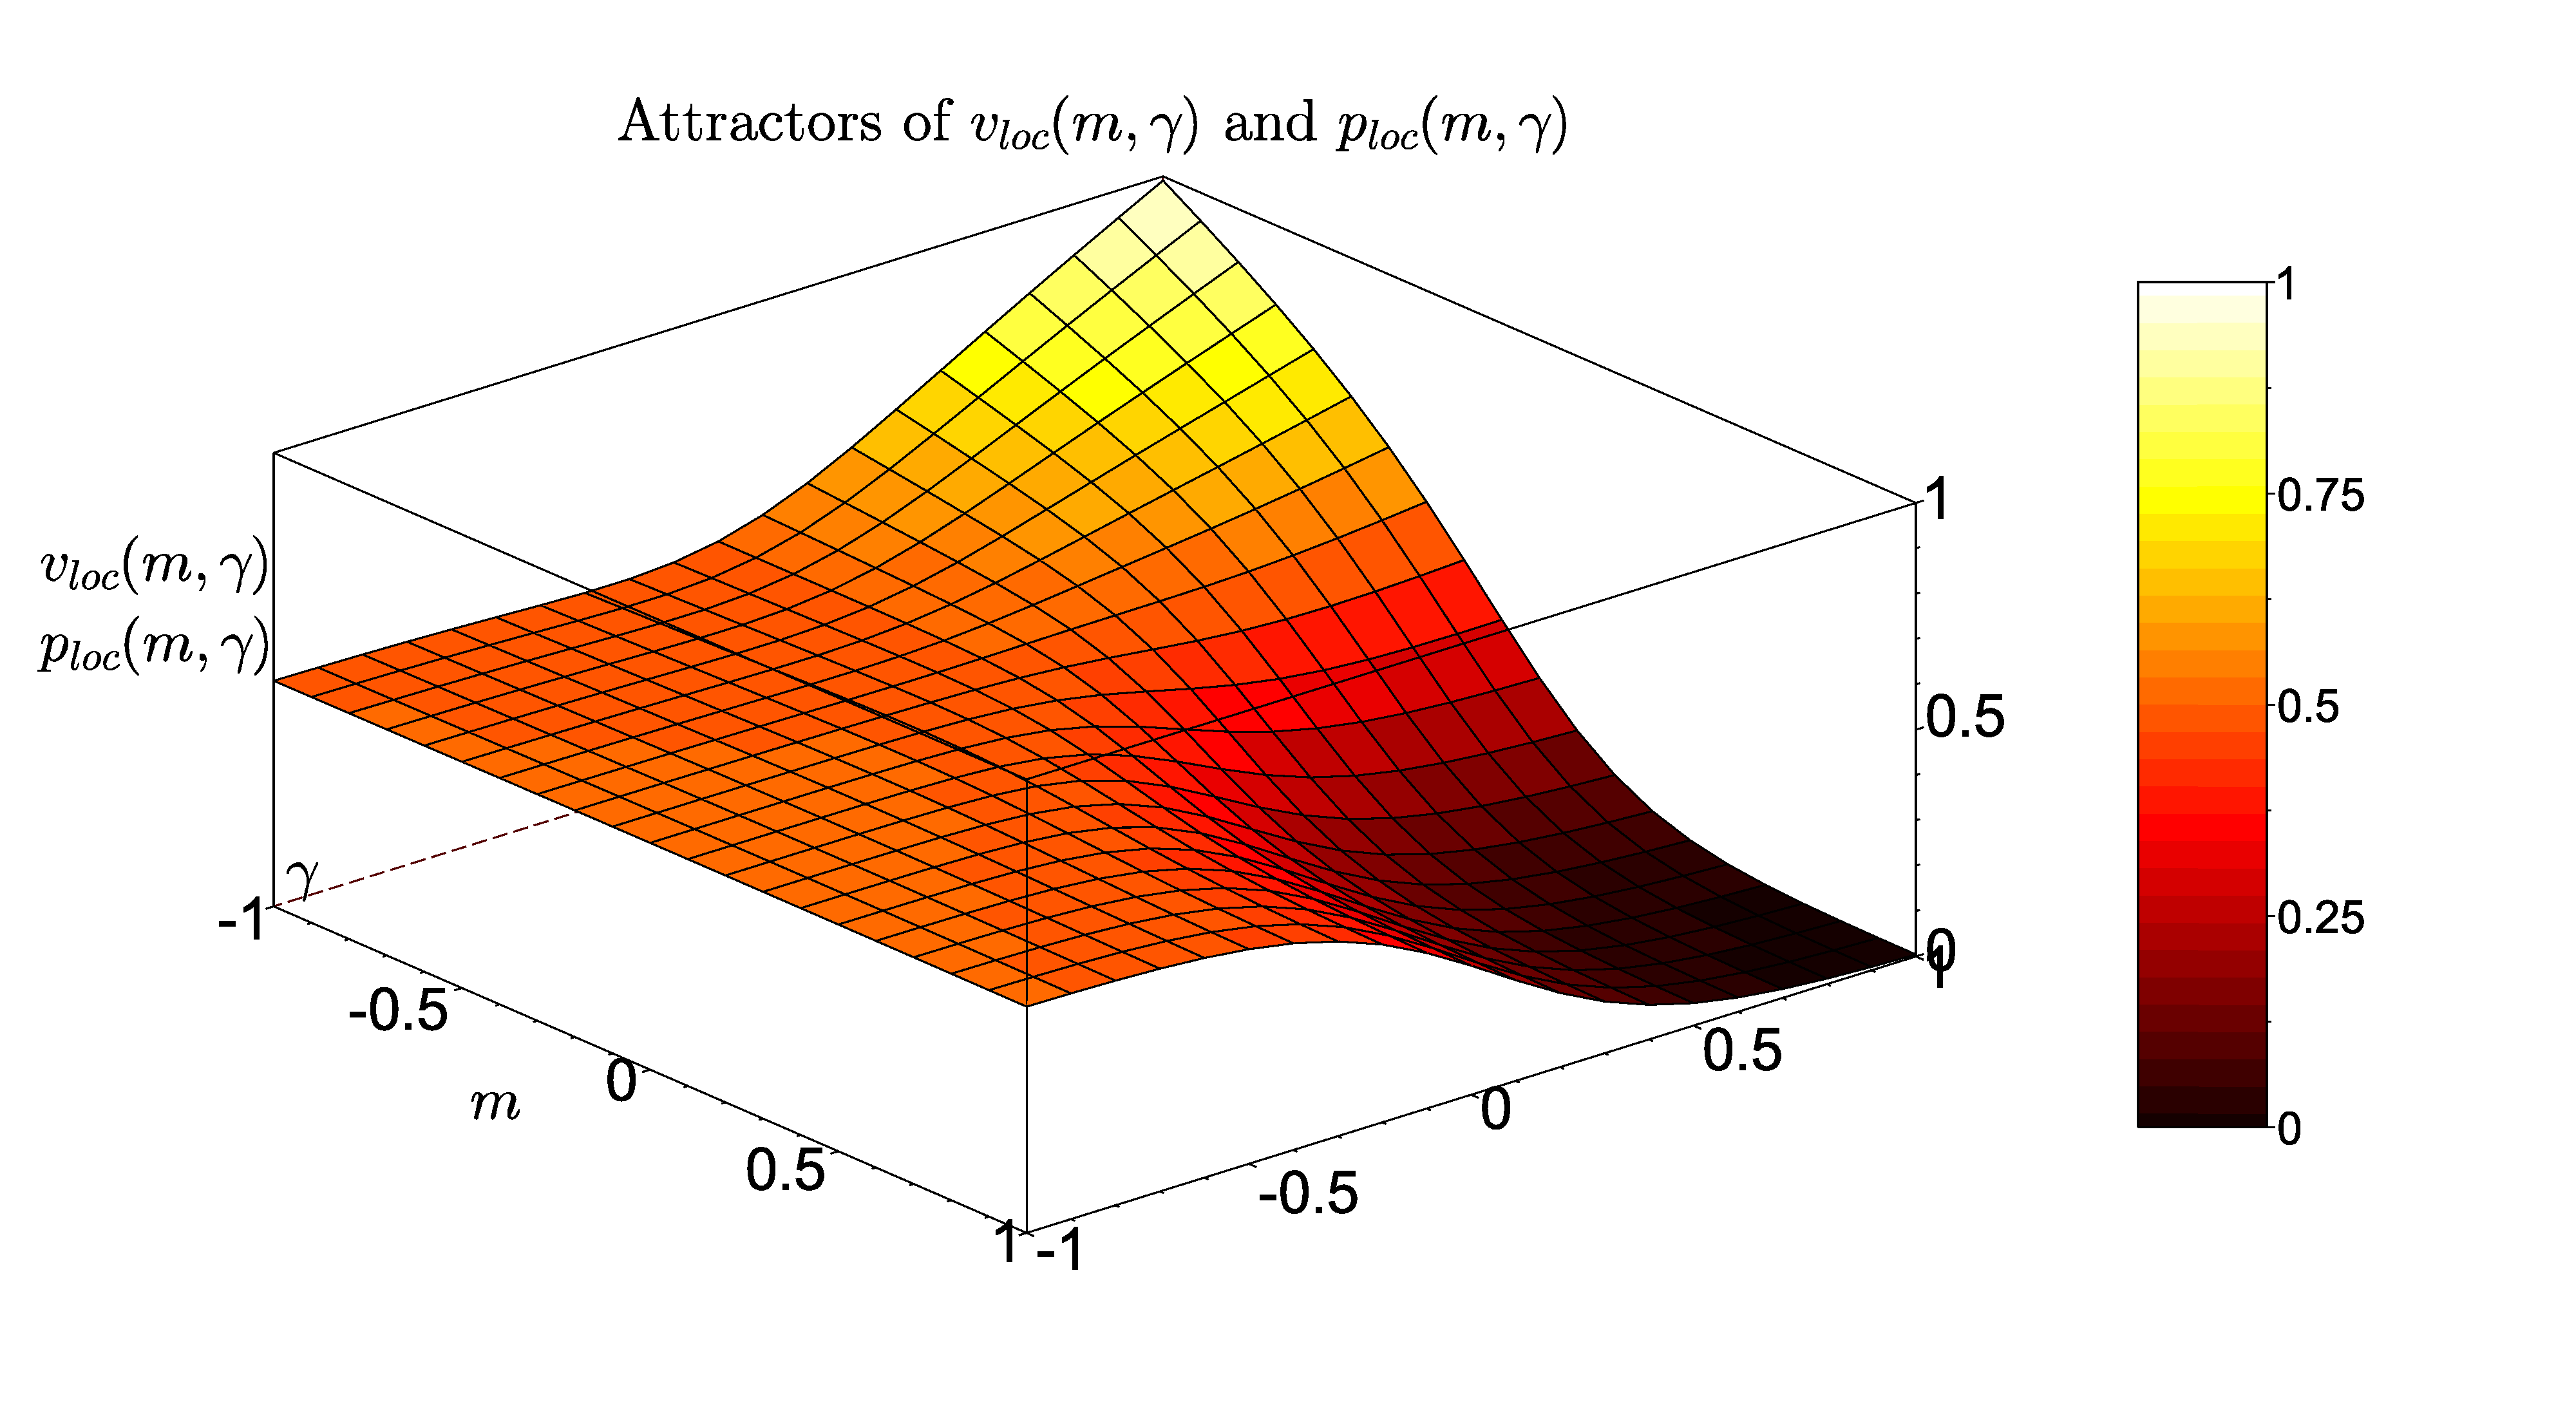
\includegraphics[width=\linewidth]{figure/bifurcProsodyLoc.pdf}
\caption{Values of $v_{loc}$ and $p_{loc}$ as functions of $m(t)$ and $\gamma(t)$.}
\label{fig_pro_loc}
\end{figure}

\begin{figure}
\centering
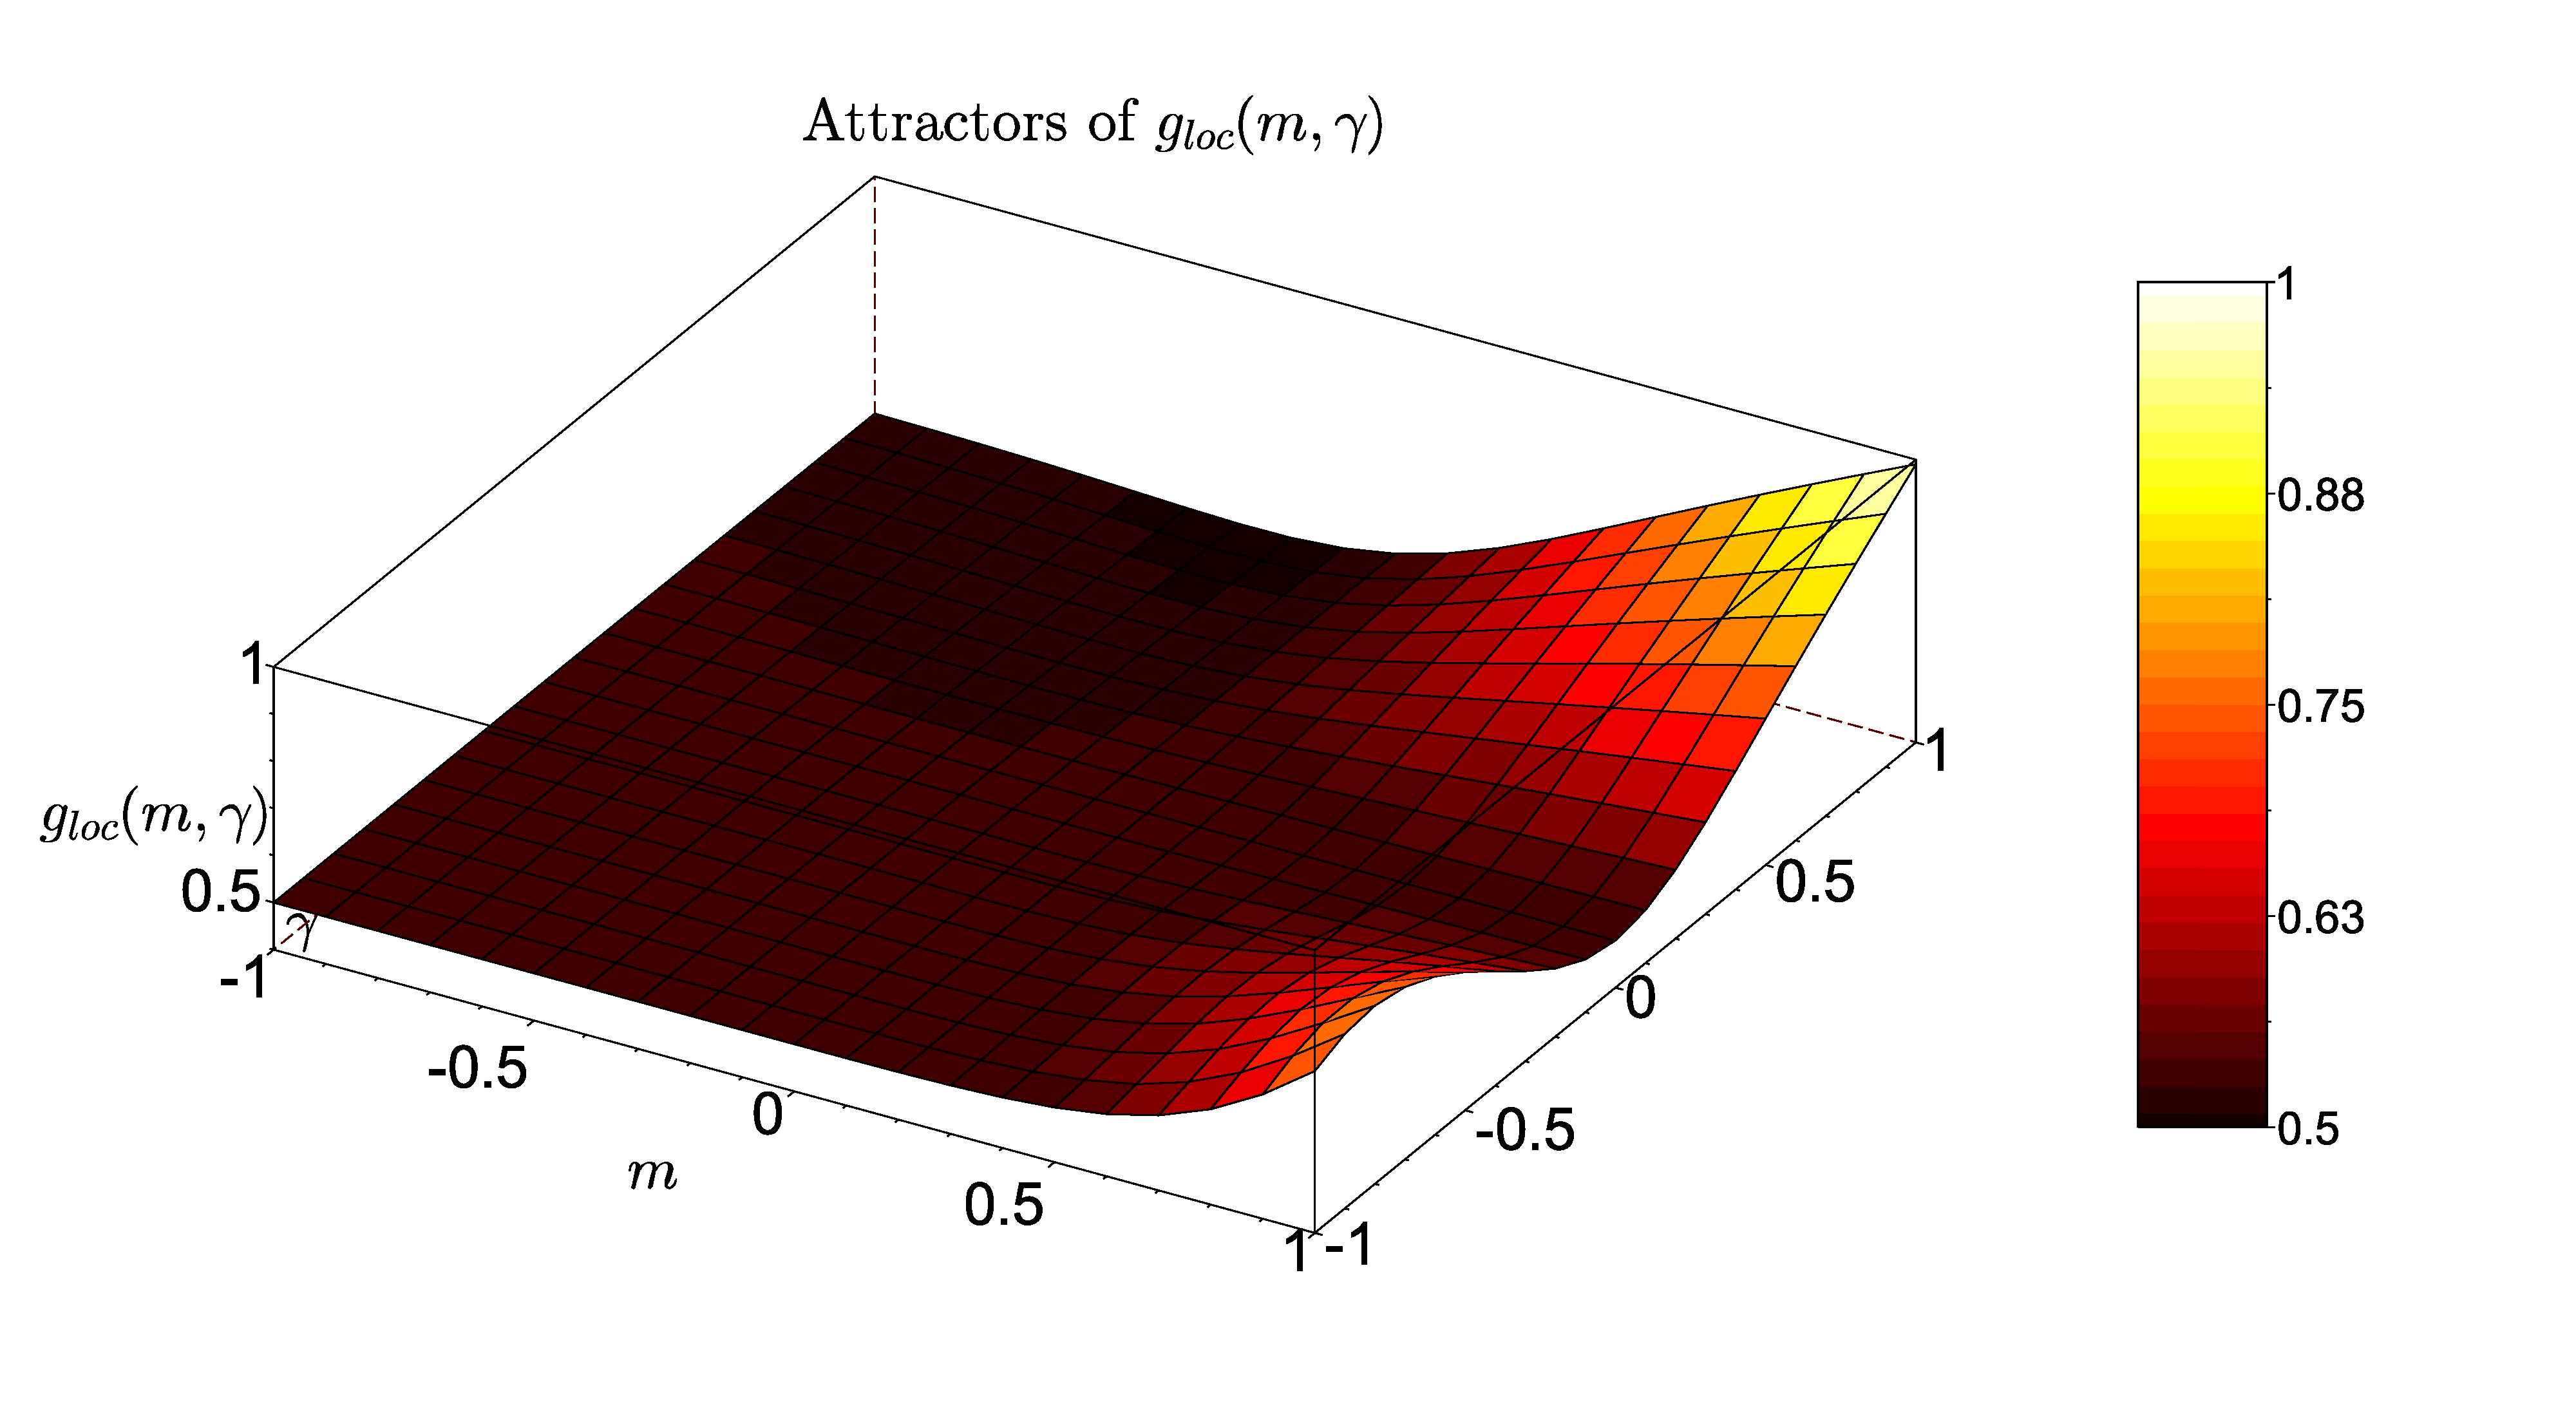
\includegraphics[width=\linewidth]{figure/gazeLoc.pdf}
\caption{Values of $g_{loc}(m,\gamma)$}
\label{fig_gaze_loc}
\end{figure}

%Before showing our simulations, we present here the equations used in the following to illustrate the properties of our model. The agents modulate three types of signals, loudness, pitch and gaze. The values of these signals have the same meaning as presented in section \ref{mod_pres}. A loudness value equal to $0$ indicates an agent that stopped speaking, a loudness value equal to $1$ the loudest value with which the participant can talk, and $0.5$ the agent's loudness mean value. Pitch follows the same logic except that a $0$ value means the minimal non nul value of pitch. For gaze, $1$ indicate an agent look permantently at the user, $0$ means the agent never look to the user, $0.5$ that the agent varies its gaze in order that 50 \% of time it looks at its partner and 50 \% it looks elsewhere. We define for each value the accumulation functions presented in the tables \ref{acc_functions_sp} and \ref{acc_functions_list}. 

% \begin{equation}
% \begin{array}{l l l}
% v_{loc}&=p_{loc}&=0.5 \\
% &&-0.5\times \gamma \times m \times S(-m)\times S(\gamma) \\
% &&-0.5\times S(\gamma) \times S(m)\\
% S(x)&&=\frac{1}{1+\exp(-10.0\times x)}
% \end{array}
% \label{loc_vol_pit}
% \end{equation}

% \begin{equation}
% \begin{array}{l l}
% g_{loc}&=0.5 \\
% &+0.5\times \gamma \times m \times S(\gamma) \times S(m) \\
% &-0.5 \times \gamma \times m \times S(\gamma(t) + m(t)) \times S(-\gamma) \times S(m) \\
% S(x)&=\frac{1}{1+\exp(-10.0\times x)}
% \end{array}
% \label{loc_gaze}
% \end{equation}

% $v_{loc}$, $p_{loc}$ and $g_{loc}$ corresponds respectively to the loudness, pitch and gaze variations. In each equations, $S(x)$ corresponds to the same sigmoid functions as used in the equation \ref{attr_foncs}, and serve the same goal as for the equations \ref{attr_foncs}. For example, the term $-0.5 \times \gamma \times m \times S(\gamma(t) + m(t)) \times S(-\gamma) \times S(m)$ is greater than $0$ if $\gamma(t)<0$, $m(t)>0$ and $\gamma(t)<-m(t)$. 

% The equations \ref{loc_vol_pit} and \ref{loc_gaze} has been defined such as the value of loudness and pitch when the partner doesn't display any turn-taking cues, that is, when the accumulation value is less than $0$ corresponds to the mean value $0.5$. 
% When $m(t)<0$ and $\gamma(t)>0$, the agent wants to keep its role and perceive that its partner is taking turn, it then increases its loudness and pitch and averts its gaze as observed in human conversations \citep{kurtic_resources_2013}. When $m(t)>0$ and $\gamma(t)>0$, the agent wants to yield its turn and perceives that its partner is taking turn, he then decreases its volume and pitch values and look towards its partner similar to what happens in human conversations \citep{gravano_turn-taking_2011,novick_coordinating_1996}. 

For the listener, the functions governing the variation of the attractor of Equation \ref{signal_control} are as follows:
 
\begin{equation}
f_{v_{lis}}= f_{p_{lis}} = \frac{1}{2} \gamma S(m+\gamma) + S(m+\gamma)S(m)S(-\gamma)
\label{lis_pro}
\end{equation}

\begin{equation}
f_{g_{lis}} = 1 - S(m + \gamma)
\label{lis_gaze}
\end{equation}

These equations has been defined such as, when the speaker produces no cues, the values of loudness and pitch equal $0$, and the gaze value equals $1$: the listener is silent and is constantly fixing its gaze toward the speaker. 
According to these equations, when $m(t)<0$ and $\gamma(t)>0$ and $|\gamma(t)|>|m(t)|$, or when $m(t)>0$ and $\gamma(t)<0$ and $|\gamma(t)|>|m(t)|$, the listener will try to take the turn by increasing its loudness and pitch values and averting its gaze from the current speaker. Figures \ref{fig_pro_lis} and \ref{fig_gaze_lis} illustrate the distribution of the attractors of Equation \ref{signal_control}, using Equations \ref{lis_pro} and \ref{lis_gaze}.

%The formulation of these equations permit to make the agent signal control equations depending on the relationship between the motivation of the agent and the strength of the cues displayed by the agent's partner. 
Figures \ref{fig_pro_loc} to \ref{fig_gaze_lis} illustrate the dynamic interplay between the agent's intrinsic motivation and the influence of the agent's partner behavior.
During the interaction $m$ and $\gamma$ are continuously varying, which results in the continuous modulation of the agent's verbal and non verbal signals production. Because the $\gamma$ of each agent depends on the signals $s_j$ produced by the other agent, the model accounts for the coupling of the two agents. This coupling leads to an emergent path in the state space of the behavioral dynamics. The next section illustrates how the turn-taking behavior, and more generally the coordination, emerges from this complex dynamics. 

% COMMENT Pierre : ce qui est explique en dessous est 2 situations compliquees - pas facile a comprendre. Il vaut miuex le voir dans la section suivante.
%For instance, the higher the listener's motivation to change role the more it will need a strong accumulation value to begin to display turn-yielding cues. In this sense, the agent will more or less resist to the perception of the speaker keeping the turn, resulting in a conflict lasting more or less. On the opposite, when the agent has a motivation to stay listener, the higher the motivation of the agent, the more the agent will ``resist" to the perception of its partner yielding its turn by staying listener. In this case, if the accumulation value is sufficiently high compared to the motivation of the agent, the agent will take the turn, as if it was forced to take it. 

\begin{figure}
  \centering
  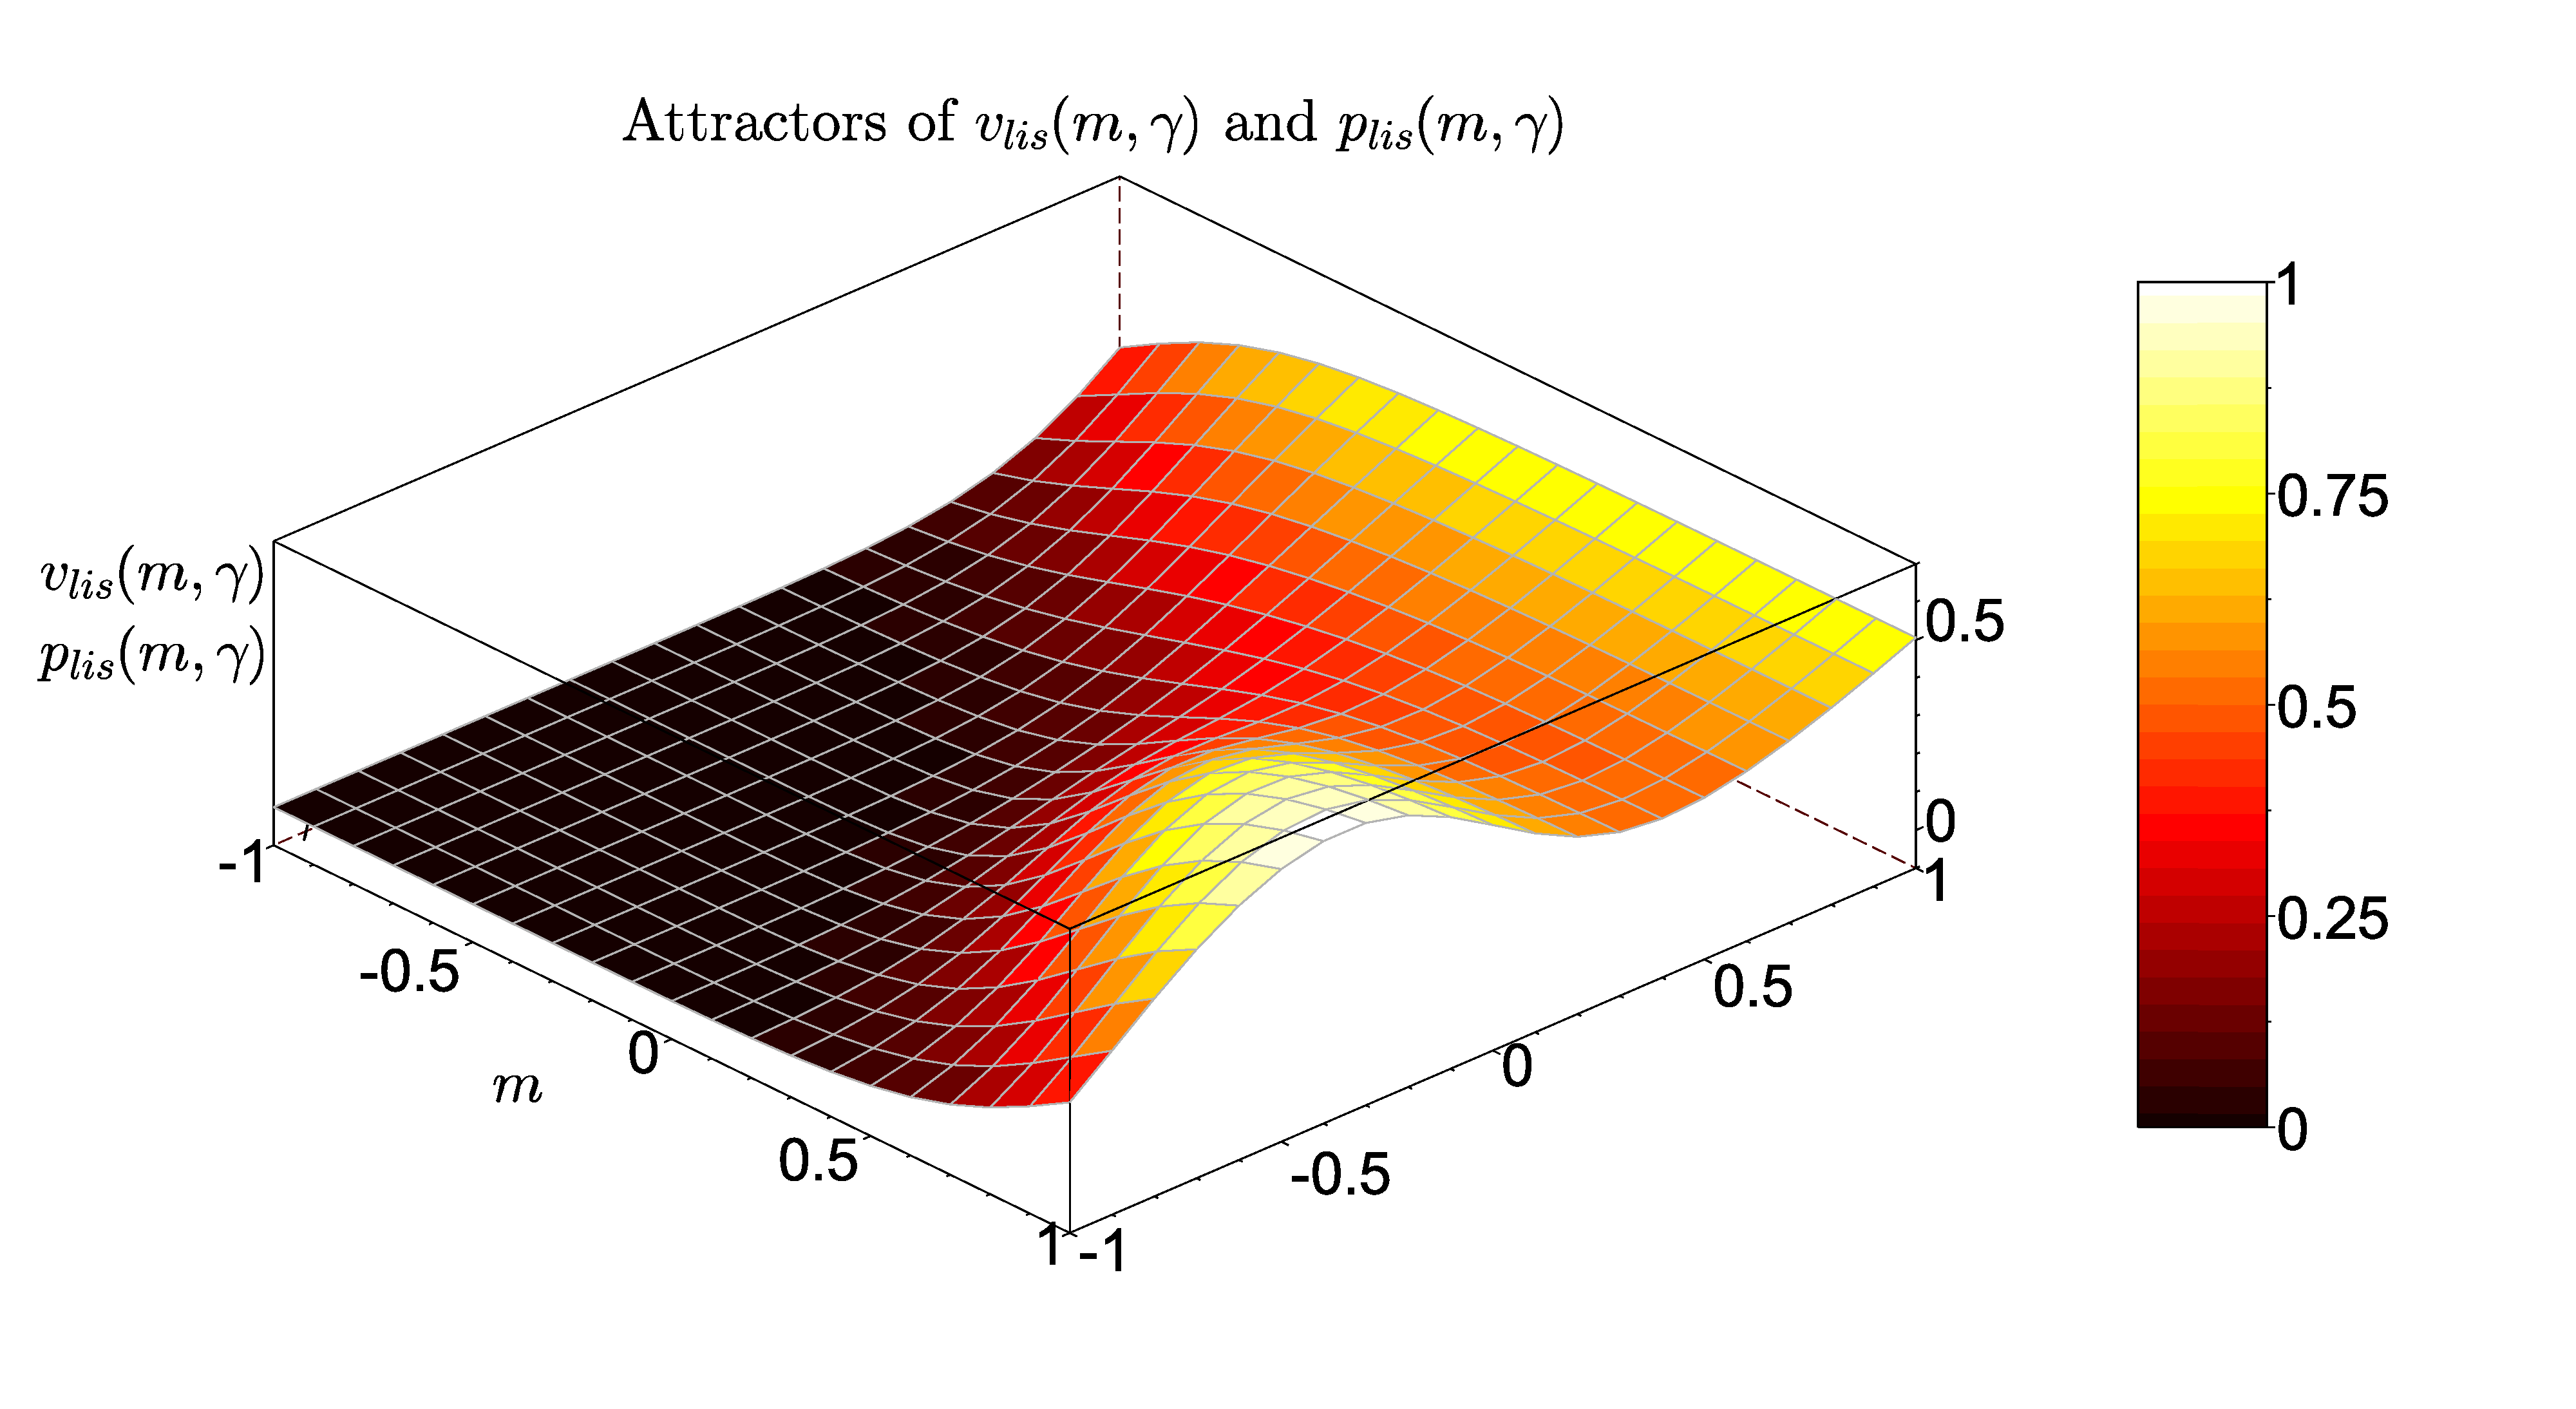
\includegraphics[width=\linewidth]{figure/bifurcProsodyLis.pdf}
  \caption{Values of $v_{lis}(m(t),\gamma(t))$ and $p_{lis}(m(t),\gamma(t))$}
  \label{fig_pro_lis}
\end{figure}

\begin{figure}
  \centering
  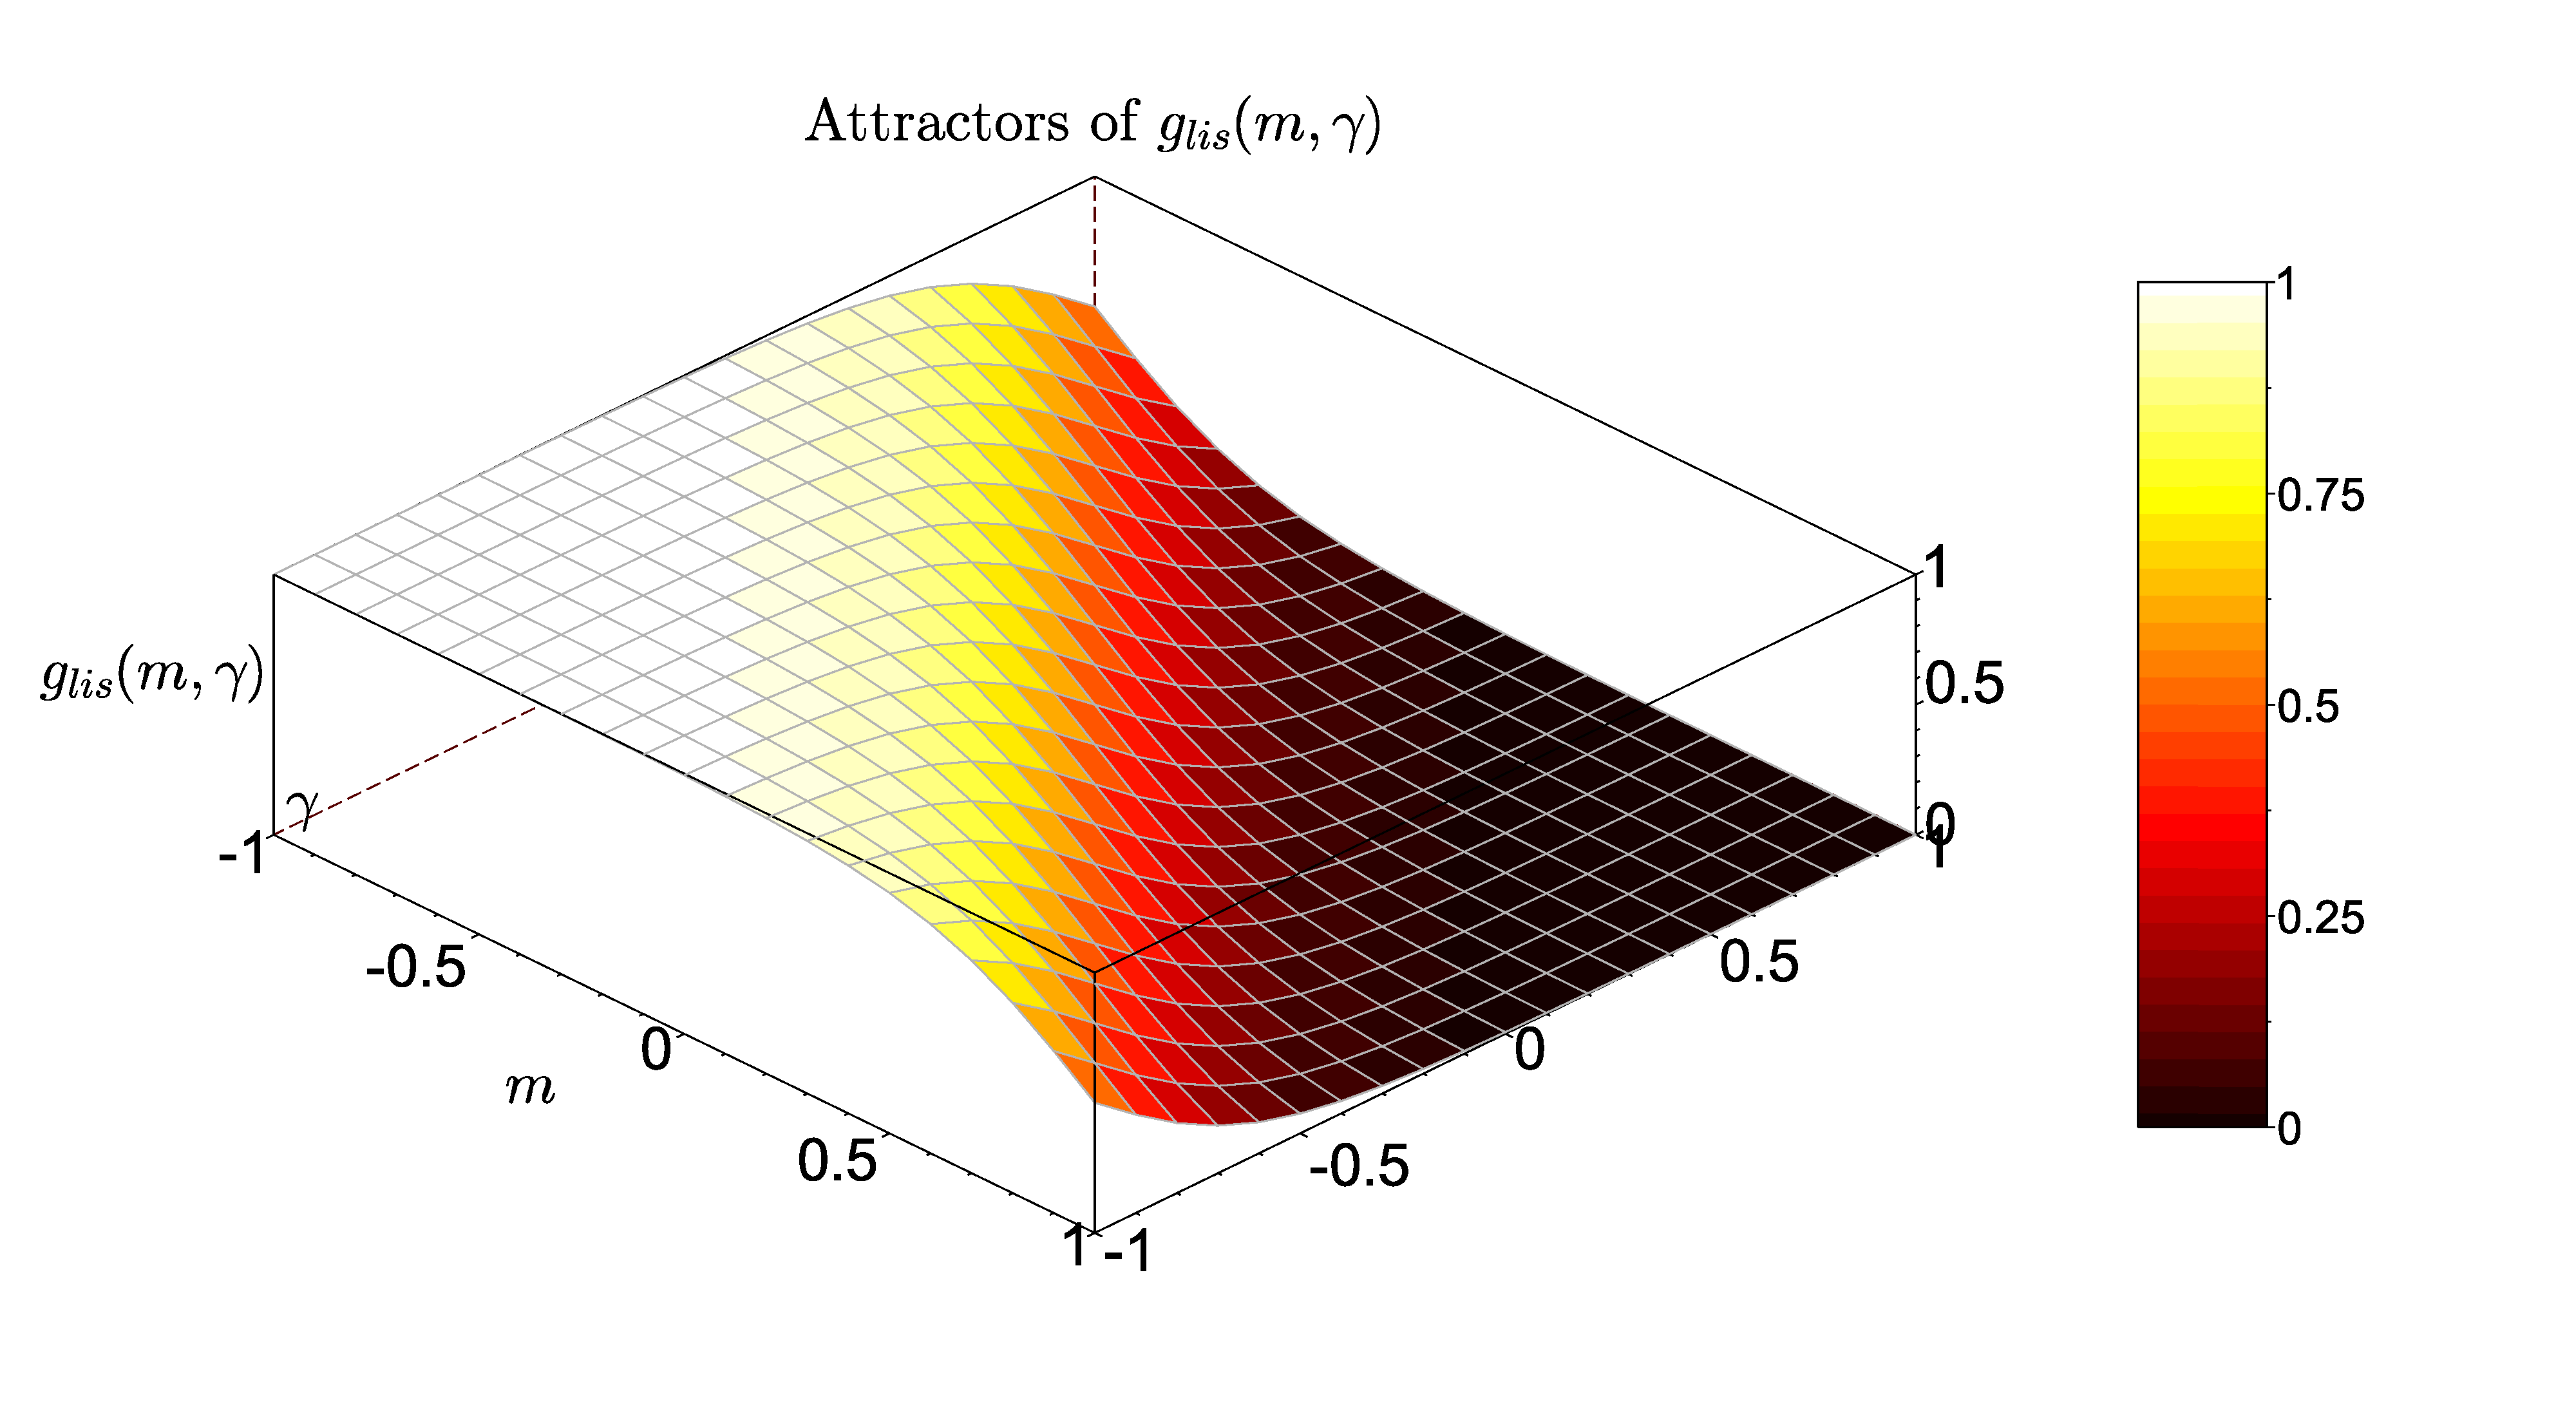
\includegraphics[width=\linewidth]{figure/gazeLis.pdf}
  \caption{Values of $g_{lis}(m(t),\gamma(t))$}
  \label{fig_gaze_lis}
\end{figure}

\subsection{Emergence of behavior}

%Based on the different theoretical equations, our aim in this section is now to show the capability of our model to make emerge the different situations linked to turn-taking. What is important about our model is the fact that the signal variations of the participants are determined not only by the motivations, that is the initial goals the participants have towards the coordination of speaking turns, either changing or keeping its role, but also directly by the accumulation value directly varying according the different signal variations of the agent's partner. As a result, we can't predict the final behavior of the agent, that is, the temporal evolution of the signal productions, but this behavior is an emergent property of the interaction between the participants. 

In the previous section, we analysed the dynamics of the state variable $\gamma$ as a response of the agent's intrinsic motivation $m$, which acts as a forcing variable of our model. In this section, we explain how the two agents coordinate their speech turns in various situations, although they are not endowed with any explicit coordination algorithm. We show that the model accounts for the different situations observed in human conversation and that the moment of time when the transition of turns occurs, or how long competitive overlaps last is not under the control any specific agent, but dynamically emerges from the interaction. Indeed, we illustrate this emergence on three contrasting scenarios, summarized in Table \ref{tab_scenarios_emergence}, that show that varying the motivation of only one of the two participants strongly change the behavior of the other participant. For sake of demonstration, in these simulations, the agents' motivation remained constant during the whole interaction. 

% COMMENT: on commence par le plus simple pour que le lecteur comprenne bien.
\begin{table}
  \begin{center}
    \begin{tabular}{ccc}
      \hline
      \mbox{} & Speaker's goal, $G_{loc}$ & Listener's goal $G_{lis}$\\
      \hline
      S3 & opposite, $m=1.0$ & strong, $m=1.0$\\
      \hline
      S4 & strong, $m=-1.0$ & strong, $m=1.0$\\
      \hline
      S5 & strong, $m=-1.0$ & low, $m=0.15$\\
      \hline
    \end{tabular}
  \end{center}
  $G_{loc}$: go on speaking (keep the same goal)\linebreak
  $G_{lis}$: say something (change to the opposite role)

  \caption{Scenarios for the analysis of the emerging behavior. Values of the forcing variable $m$ for the two agents.}
  \label{tab_scenarios_emergence}
\end{table}

\begin{figure}[b]
  \centering
  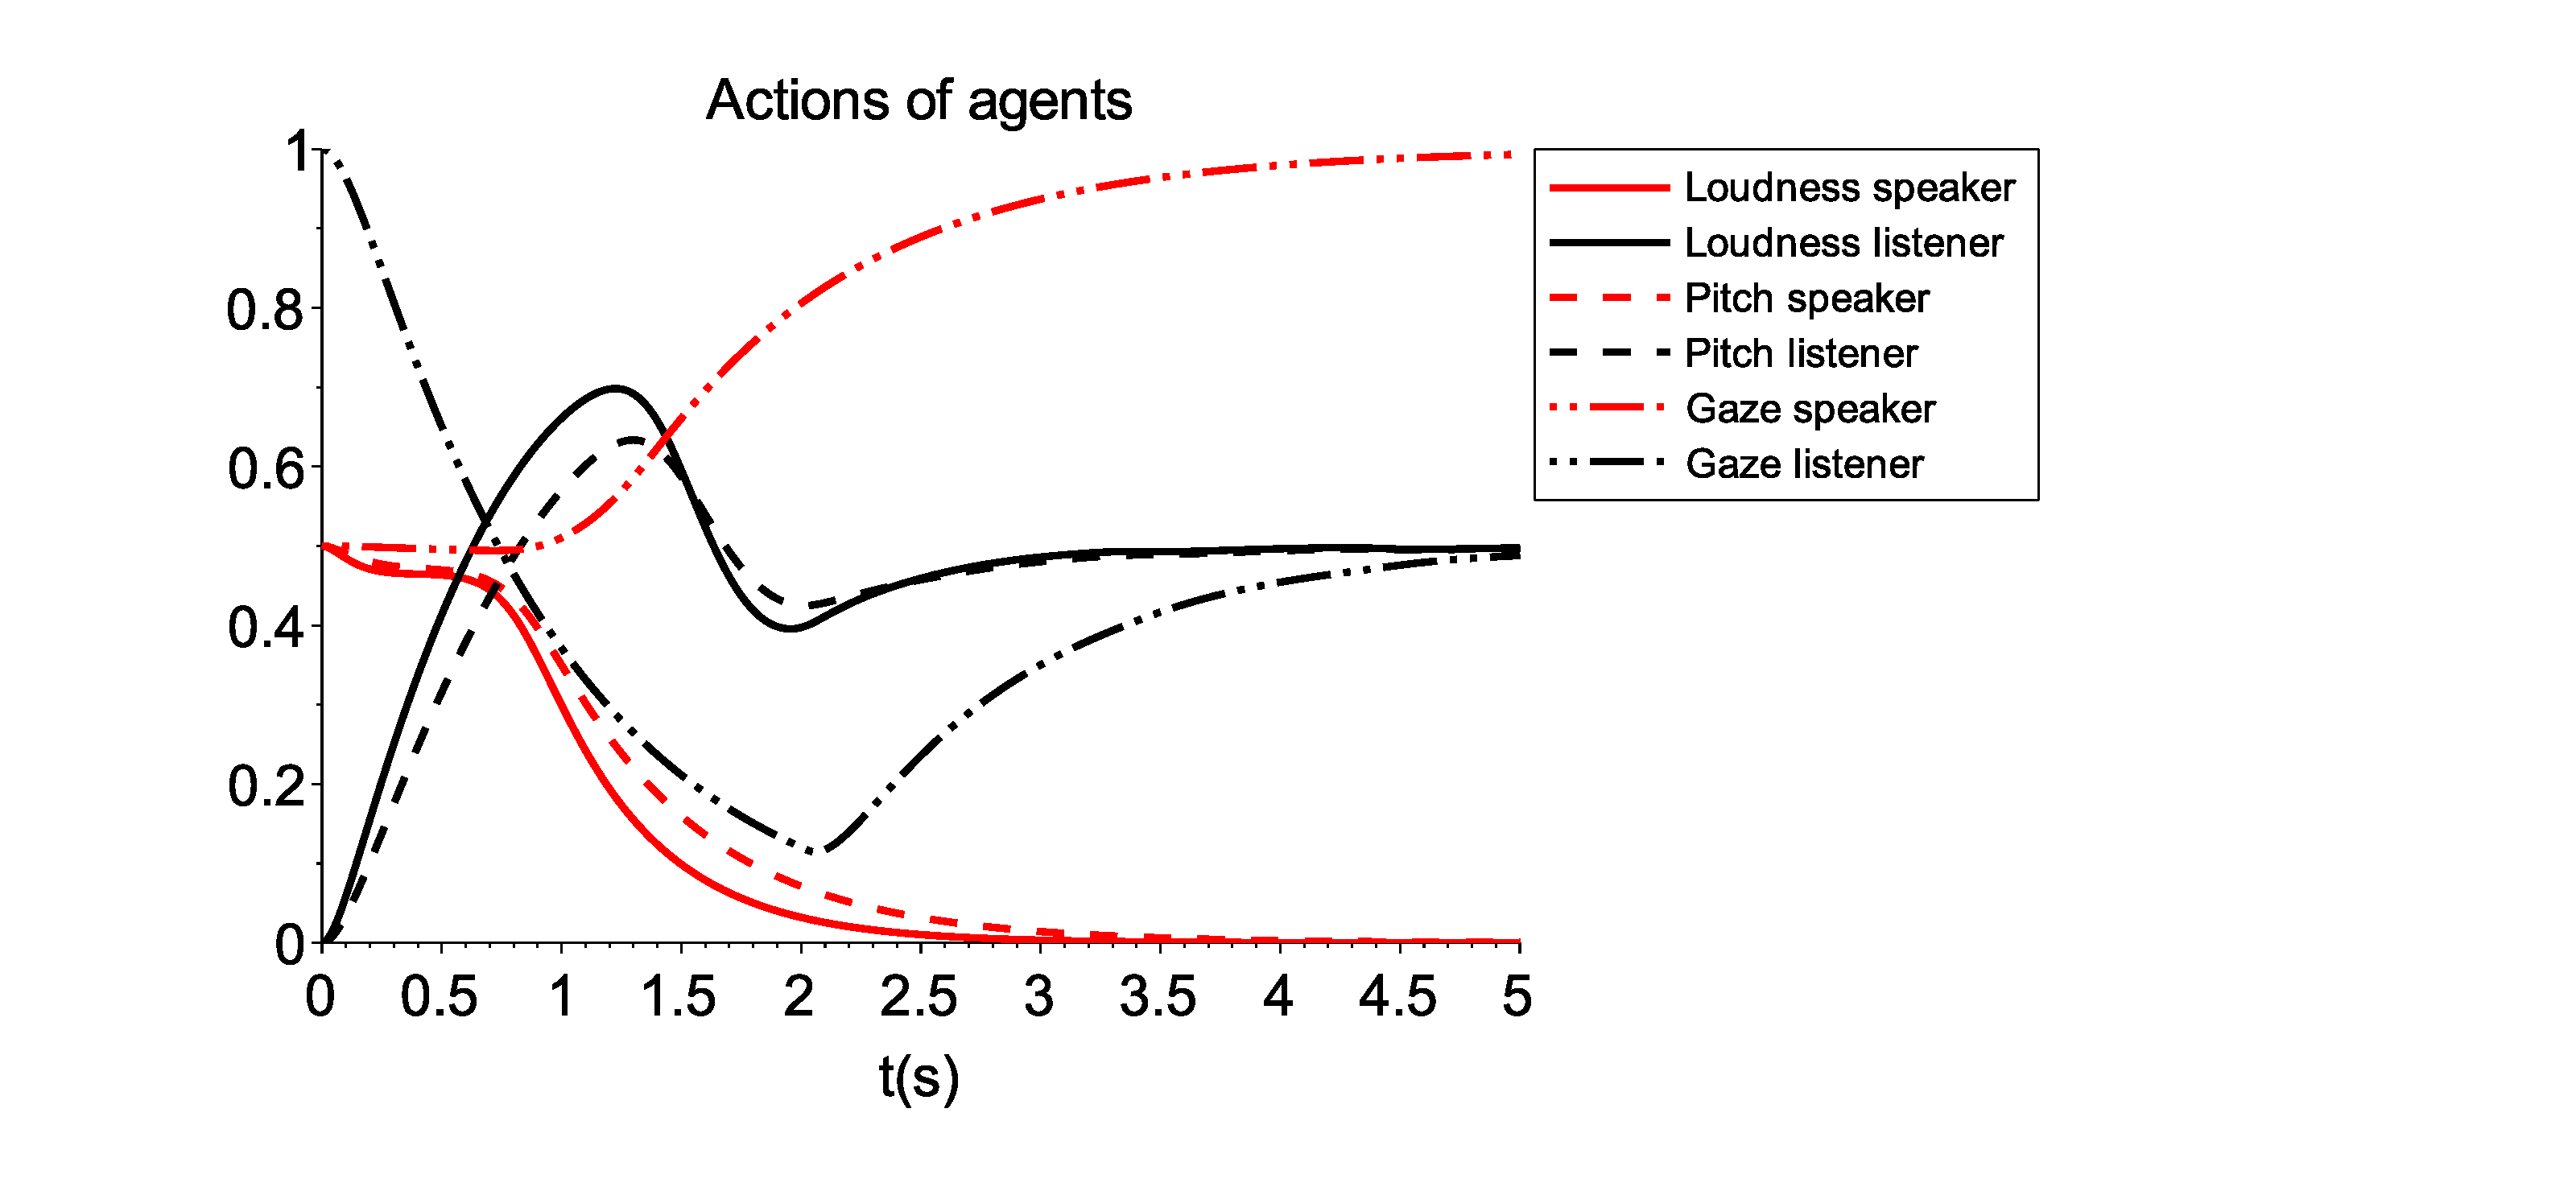
\includegraphics[width=\linewidth]{figure/smooth-transition_signal-production.pdf}
  \caption{Modulation of the verbal and non verbal signals produced by the two agents. The resulting behavior is a smooth transition of the turn from the current speaker to the current listener. Scenario S3} 
  \label{simu_smooth}
\end{figure}

\begin{figure}[t]
  \centering
  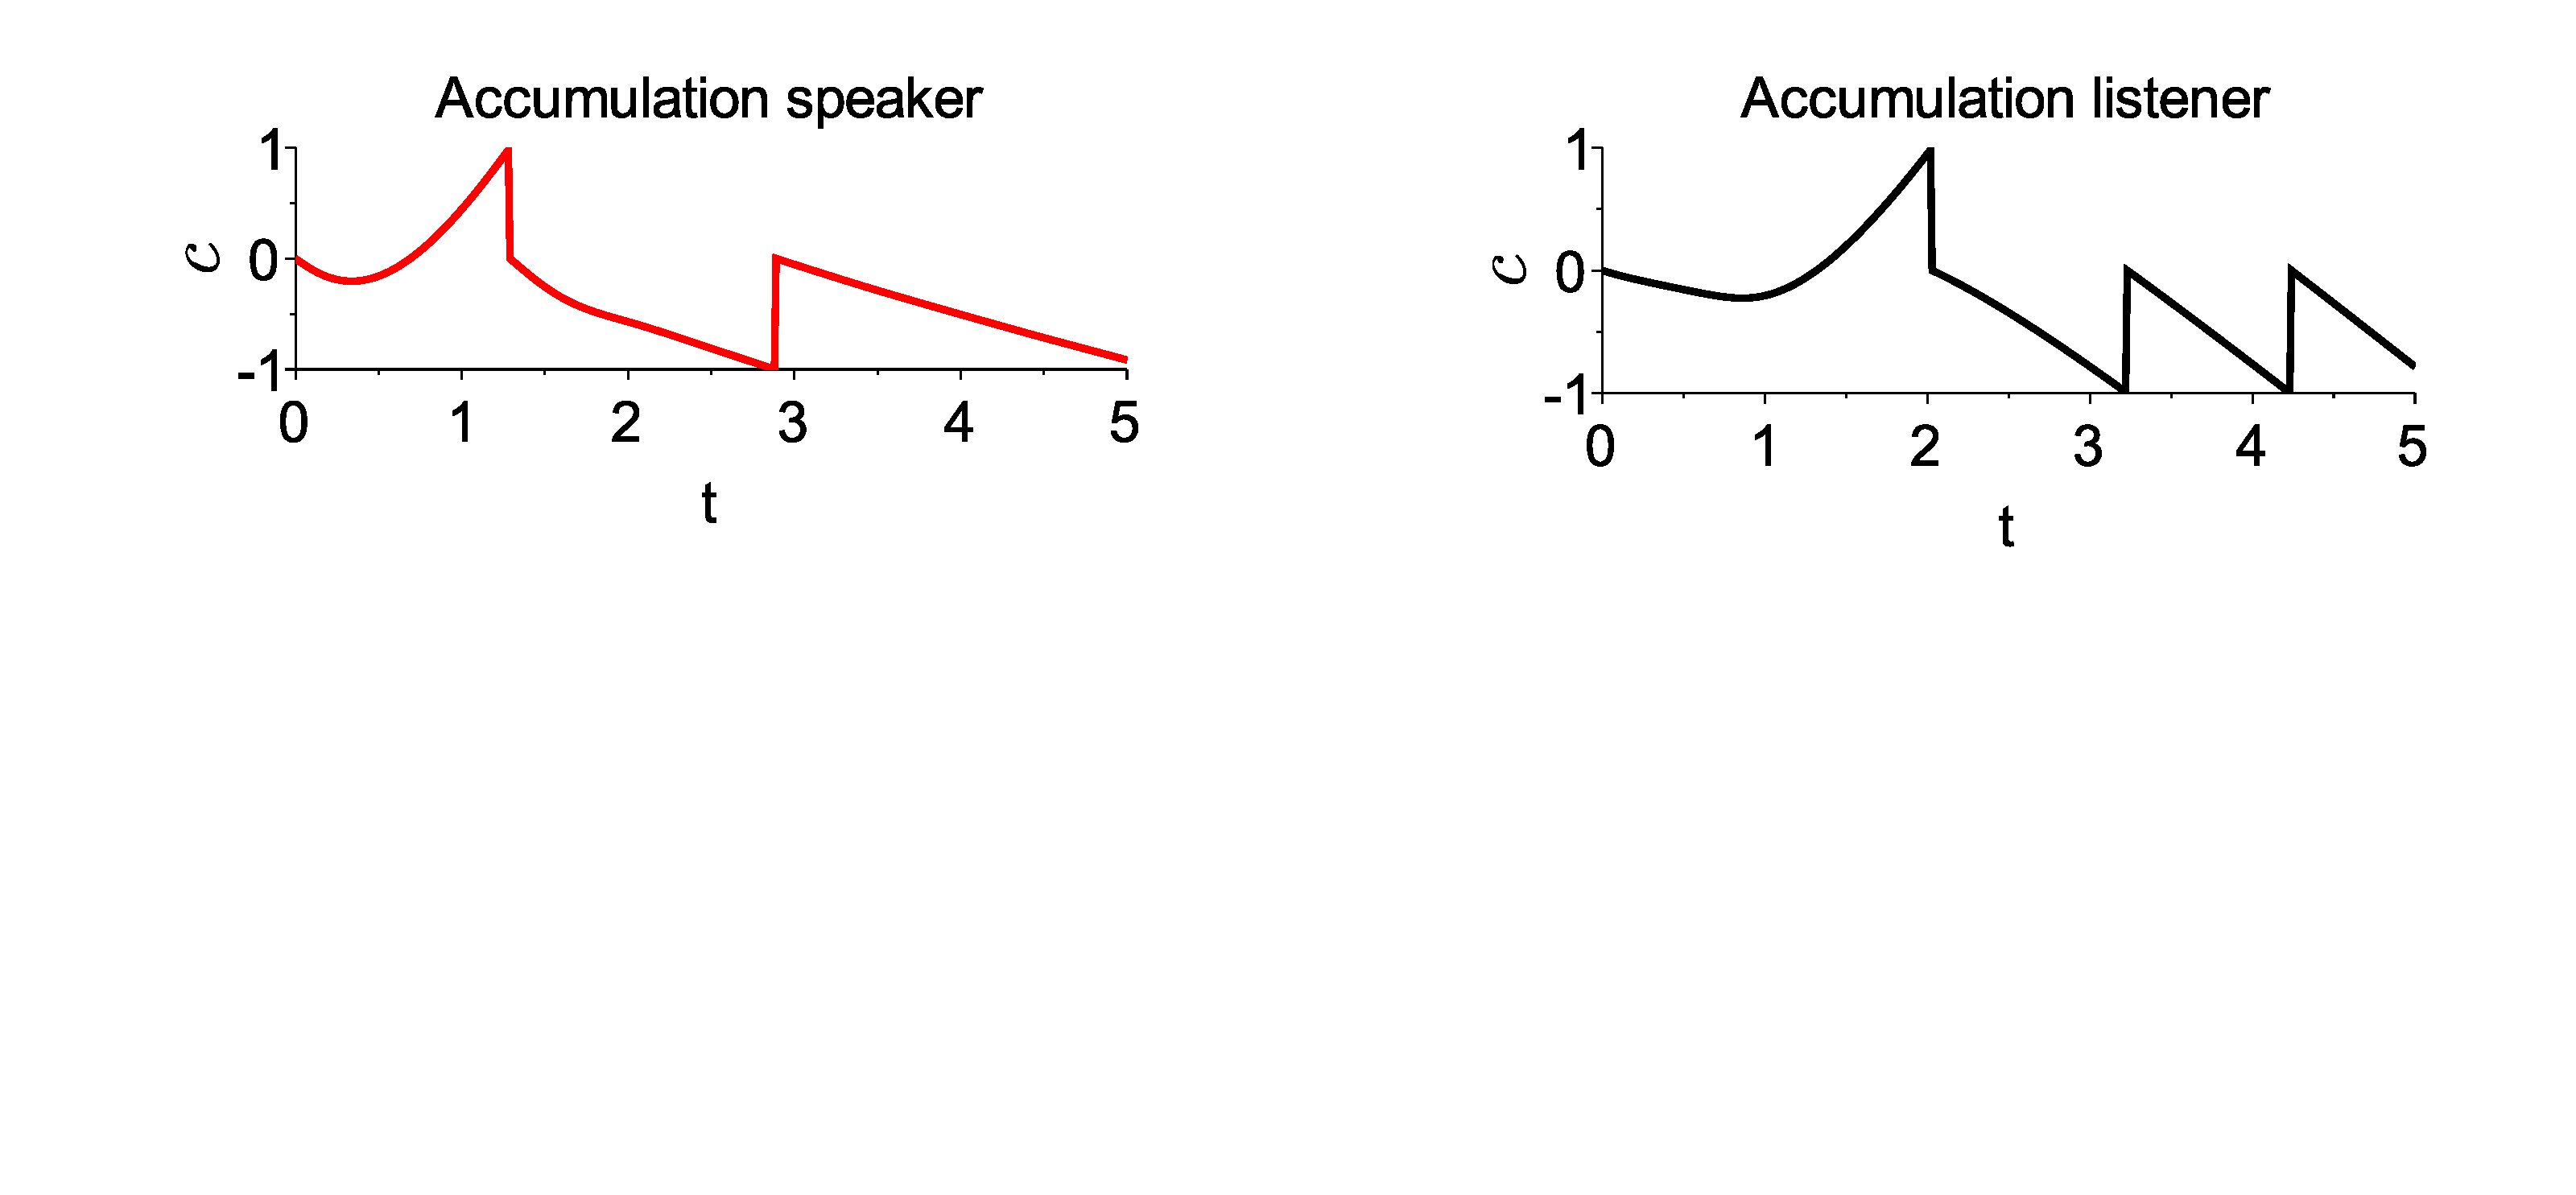
\includegraphics[width=\linewidth]{figure/smooth-transition_accumulation_small.pdf}
  \caption{Time series of the accumulation values $\gamma$ for the two agents. Scenario S3.}
  \label{smooth_acc}
\end{figure}


In scenario S3, the current speaker had a strong motivation to yield the turn and the current listener a strong motivation to take the turn. Figures \ref{simu_smooth} shows how the agents modulated their verbal and non verbal signal productions (here the loudness and the pitch of their voice, and their gaze direction). Figure \ref{smooth_acc} shows the dynamic of the perceptual decision-making process. As one could expect, the model led to a short non conflicting overlap, in the terms given by \citep{schegloff_overlapping_2000}. 

Scenario S4 shown that if we modify the current speaker's motivation, we impact the behavior of the two agents. In S4, the current speaker had a strong motivation to go on speaking and the current listener a strong motivation to take the turn. The result of this simulation is shown on Figure \ref{simu_interruption} and  Figure \ref{inter_acc}. In this situation, the model reproduced a conflicting overlap, which ended by the initial listener holding the floor.  

\begin{figure}
  \centering
  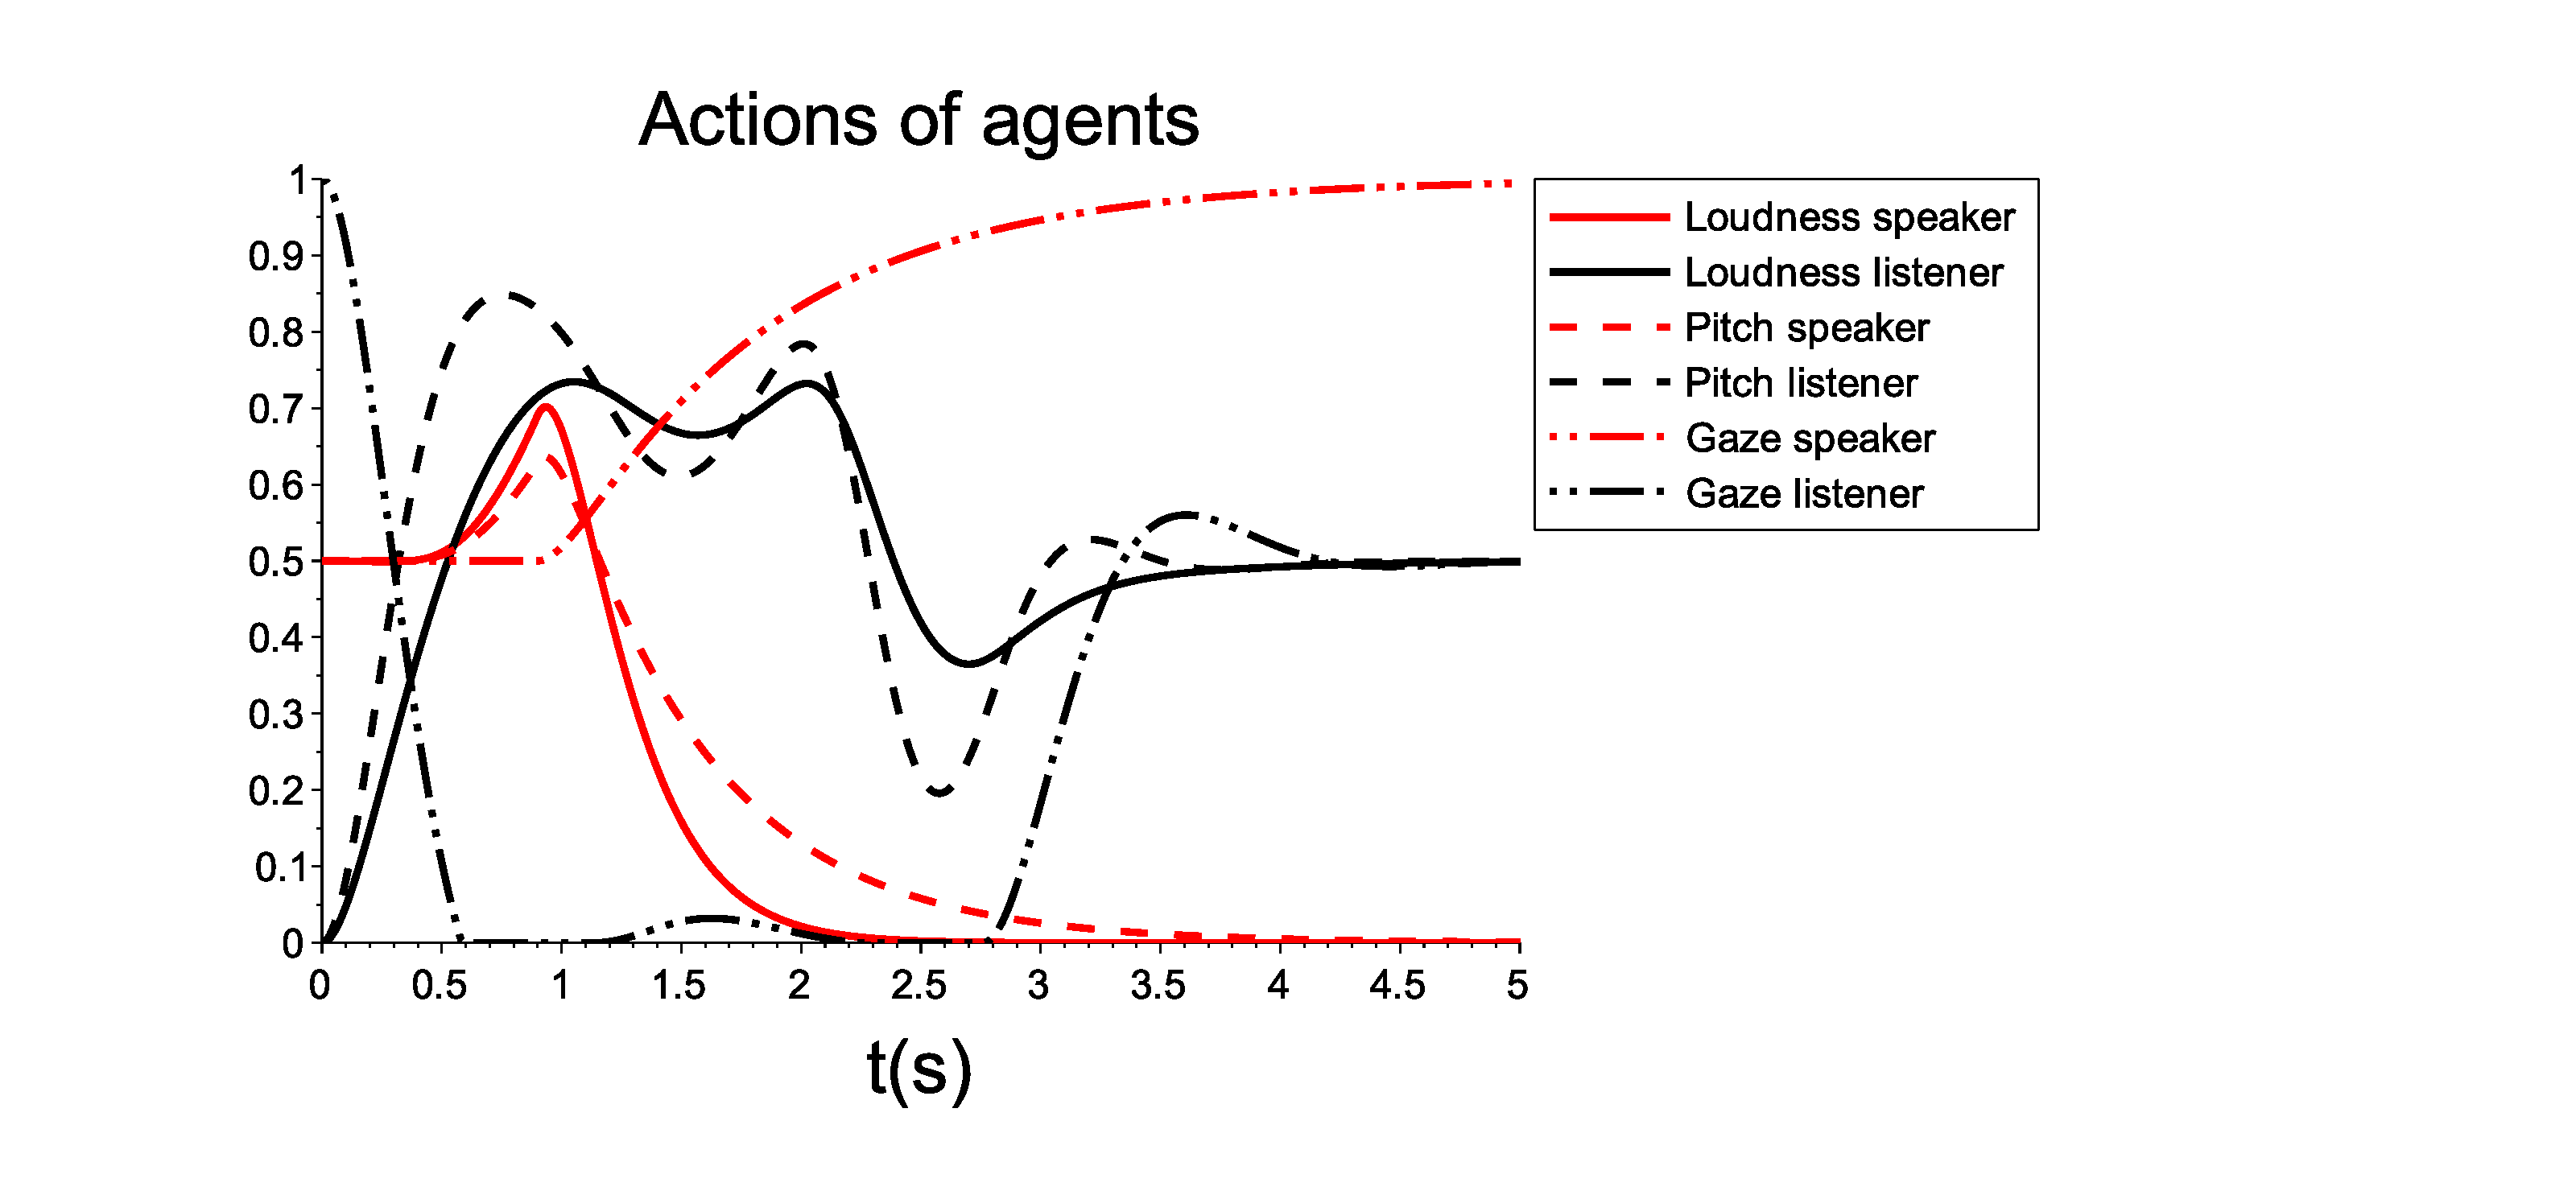
\includegraphics[width=\linewidth]{figure/emerg_sc1.pdf}
  \caption{Modulation of the verbal and non verbal signals produced by the two agents. Scenario S4. The resulting behavior is a conflicting overlap lasting about 2 seconds.}
  \label{simu_interruption}
\end{figure}

\begin{figure}
  \centering
  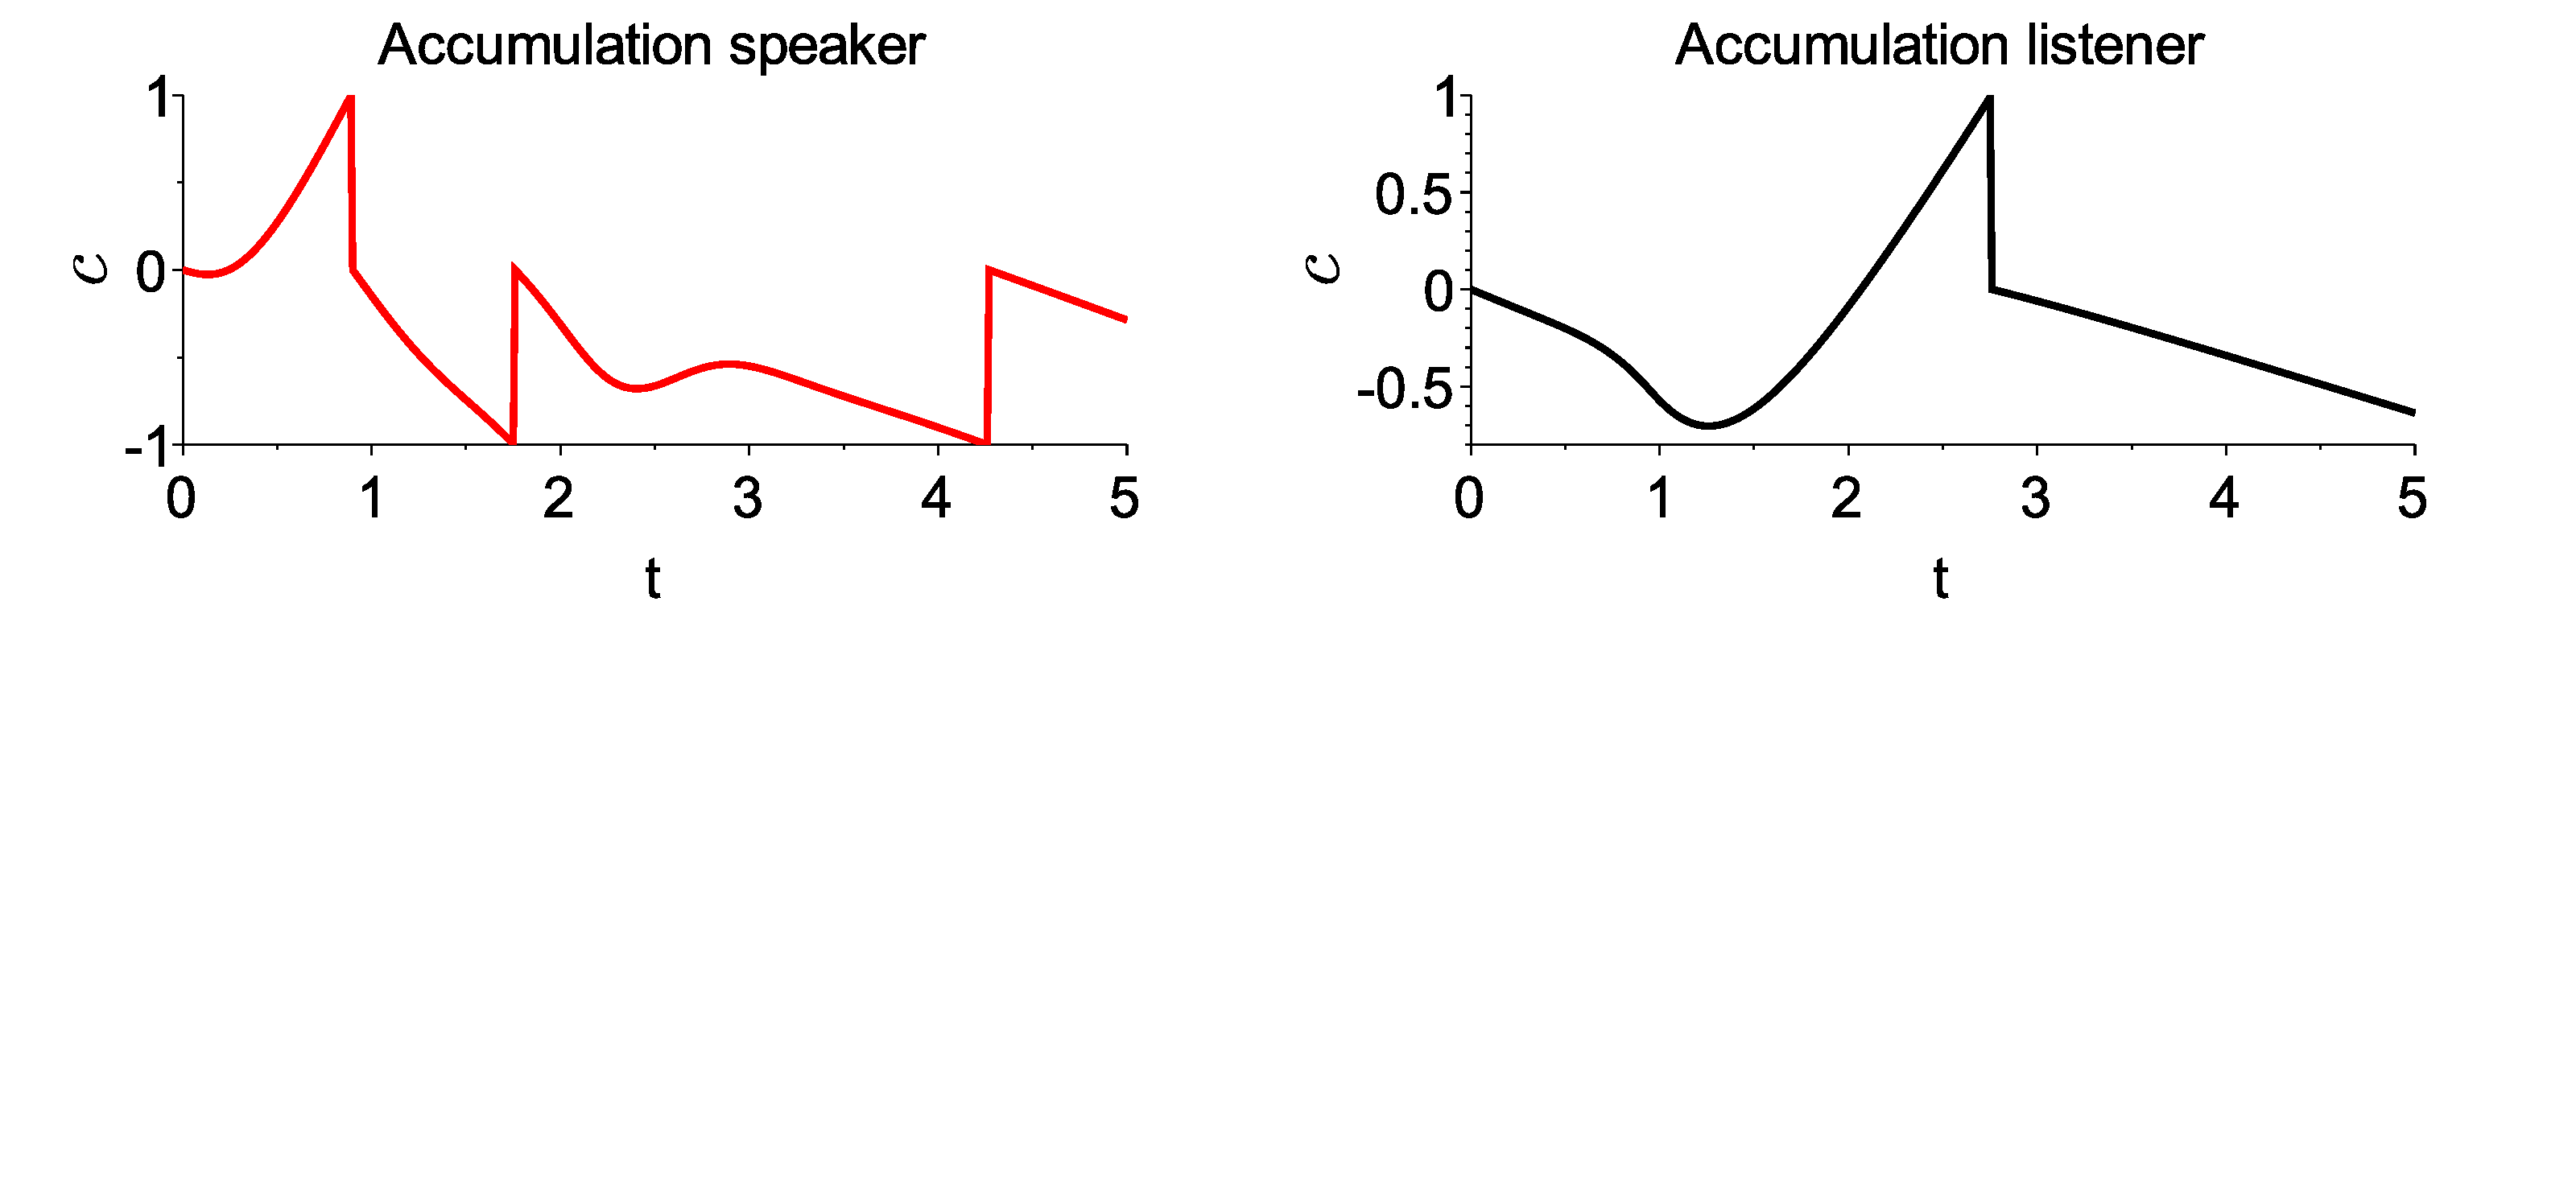
\includegraphics[width=\linewidth]{figure/acc_sc4_small.pdf}
  \caption{Time series of the accumulation values $\gamma$ for the two agents. Scenario S4.}
  \label{inter_acc}
\end{figure}

This scenario shows the continuous dependency of each participant to the signals production of the other one. At the beginning of the simulation, the current speaker was keeping its voice loudness to its mean value $0.5$. As its accumulation value raised, due to the raise in the loudness and pitch of the current listener, at $t\approx~750~\text{ms}$ the current speaker raised its own prosodic variables and averted its gaze, showing to the current listener its willingness to remain the speaker. Nevertheless, the modulations of the current speaker's signals (as defined by the equations governing the signal production) weakly impacted the signals production of the current listener. As a result, the current listener was continuing to try to take the turn, the accumulation value of the current speaker crossed the positive threshold, and the current speaker finished to yield the turn to the current listener. In turn, the current listener diminished its loudness and pitch, perceiving that the previous speaker finished to yield the turn, which finally ended the conflictual situation.

If we now keep the same motivation value for the current speaker but we diminish the motivation of the current listener we obtain a completely different behavior for the two agents, as shown by Figures \ref{simu_buttin} and \ref{acc_buttin}, corresponding to scenario S5. We illustrate here the speaker's successive but unsuccessful attempts to yield the turn. The choices made in the specific equations used for these simulations are responsible for the way the conflict is here resolved.  

\begin{figure}
  \centering
  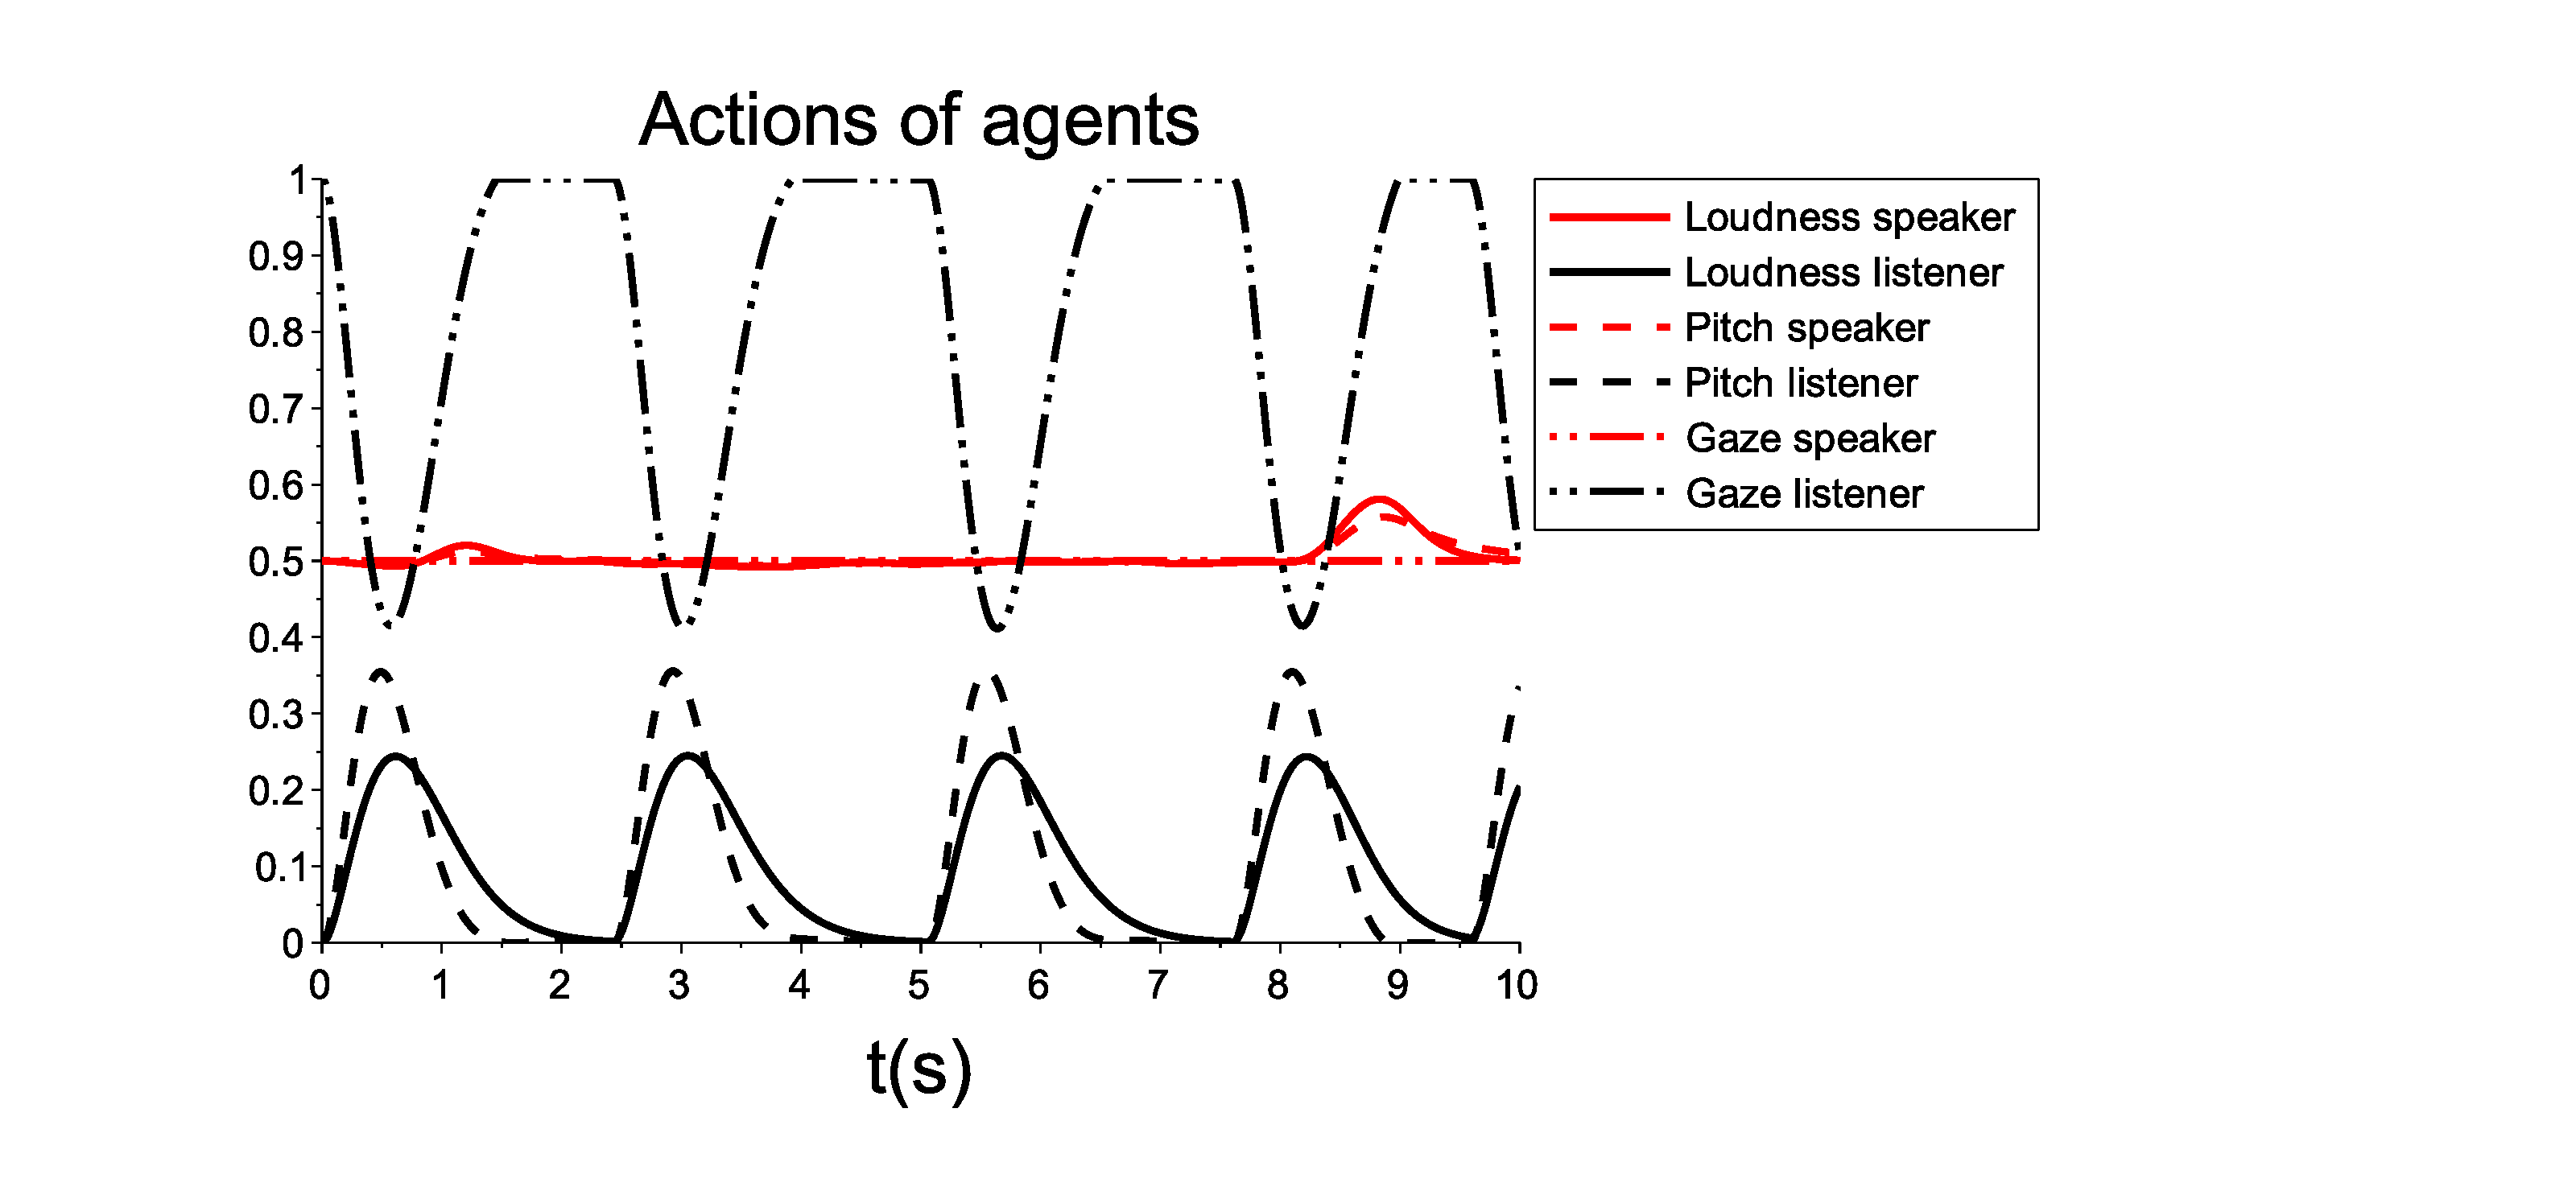
\includegraphics[width=\linewidth]{figure/emerg_sc2.pdf}
  \caption{Modulation of the verbal and non verbal signals produced by the two agents. Scenario S5.}
  \label{simu_buttin}
\end{figure}

\begin{figure}
  \centering
  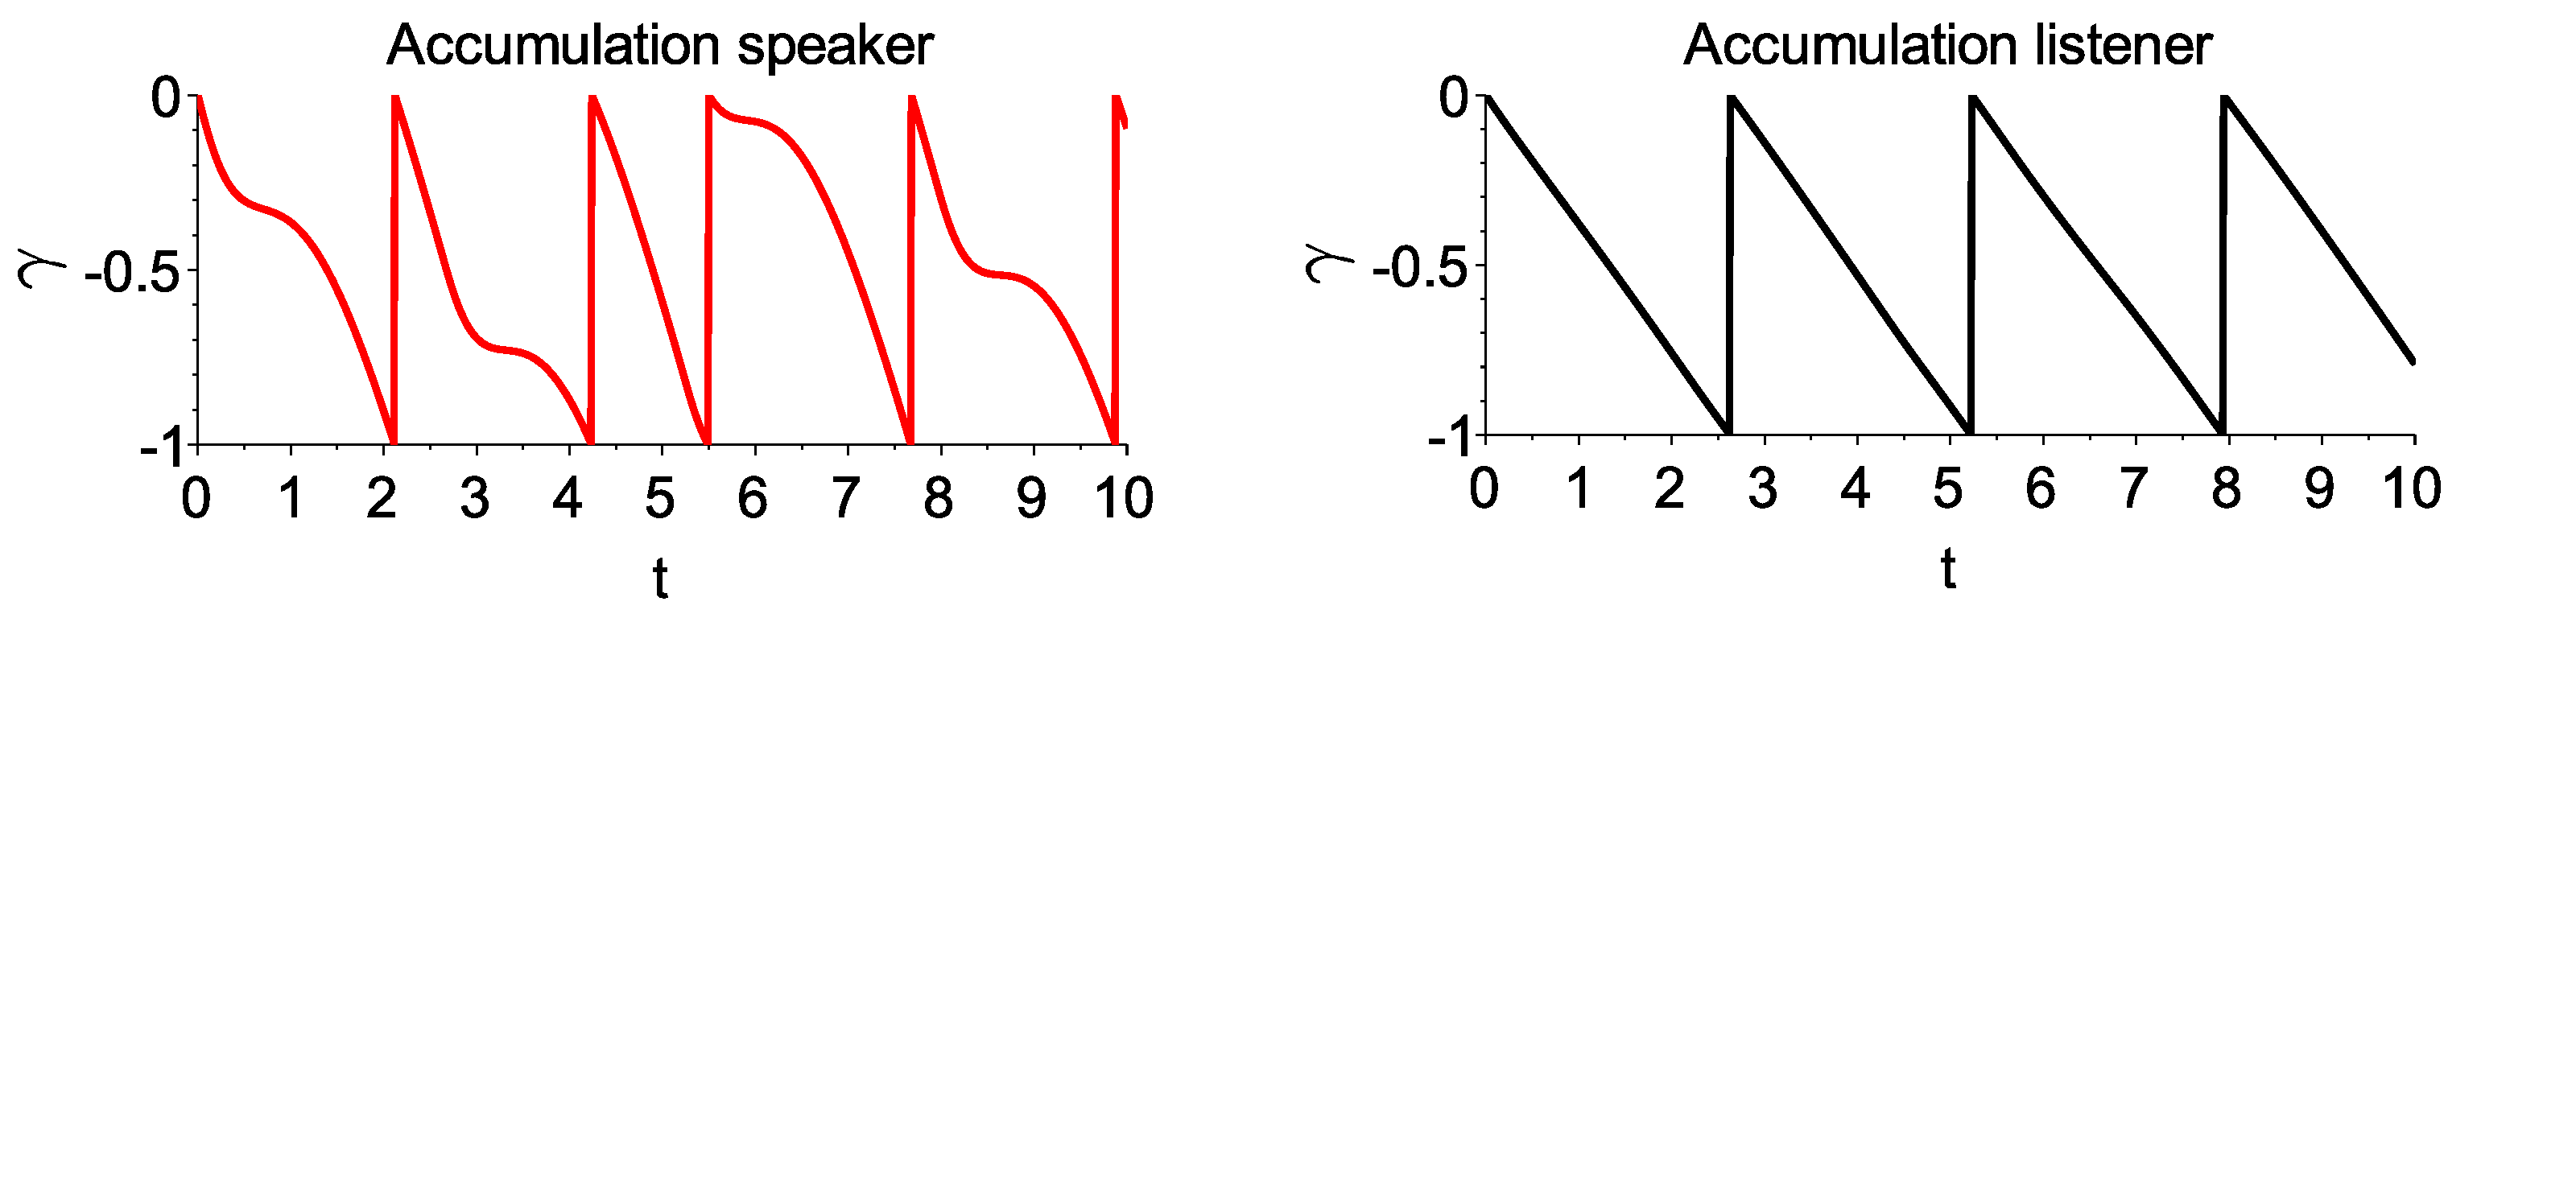
\includegraphics[width=\linewidth]{figure/acc_sc2_small.pdf}
  \caption{Time series of the accumulation values $\gamma$ for the two agents. Scenario S5.}
  \label{acc_buttin}
\end{figure}

In S5, the current speaker succeeded to keep its role in spite of the several turn-taking attempts of the current listener. This was because the motivation of the current listener was weaker than previously, meaning that it gave up more rapidly when it observed no cues indicating that the current speaker was yielding the turn. At the beginning of the simulation, the accumulation value of the current speaker raised, resulting in a current speaker averting its gaze from the listener. As the current listener gave up, the accumulation value of the current speaker diminished again, resulting in a gaze control parameter returning to the value $s_g=1$, meaning that the agent was fixing its partner. The fact that the loudness and pitch did not vary was simply due to an accumulation that was not high enough for the prosodic signals to raise. In other terms, the agent did not need to raise its prosodic signals to prevent the current listener to take the turn. The observed repetition of the turn-taking attempts of the current listener was due to the fact that, as defined in section \ref{mod_pres}, when the accumulation value crosses the negative threshold, the accumulation process is reinitialized. Thus the current listener became again uncertain about the behavior of the current speaker, and thus initialized a new turn-taking attempt. 


These three simulations show that the resulting behavior of each participant is not solely determined by their motivation value, but is also indirectly impacted by the motivation of the other participant. In this sense, a sensorimotor coupling is established between participants, as the action variations of one participant directly impact the modulation of the actions of the other participant, resulting in a very versatile coordination. Since both participants continuously influence the other's behavior, one cannot predict in advance the resulting behavior of the two participants. These behaviors are then an emergent property of the interaction of the two participants. 

\subsection{Adaptability of the behavior}

The behaviors of the two participants emerge from the interaction. But, what benefits bring this sensorimotor coupling between both participants?
We show in this section, how this sensorimotor coupling can explain how participants can seamlessly adapt to different environmental settings without modifying the different equations governing the perceptual decision-making process and the production of the verbal and non verbal signals. We will show this adaptability on examples where we varied the number of signals the agents can handle. 

% ------------------------------------------------------------------------------
%\subsubsection{Adaptability to the amount of information}

The different analyses conducted in this section have been performed using scenario S5 (see table \ref{tab_scenarios_emergence}) and a variant S6, where the agents did not use the direction of gaze of their partner in the perceptual decision-making process. 
These two scenarios correspond to a conflicting situation when the current listener makes several unsuccessful attempts to take the turn, the current speaker averting its gaze in response to the turn-taking attempt. Figure \ref{simu_buttin} illustrates the signal production of the two participants when they perceived the totality of the signals produced by the other participant (S5). Figure \ref{adapt_nogaze} illustrates what happened when agents did not have access to the gaze direction of their partner (S6).

% \begin{figure}
%   \centering
%   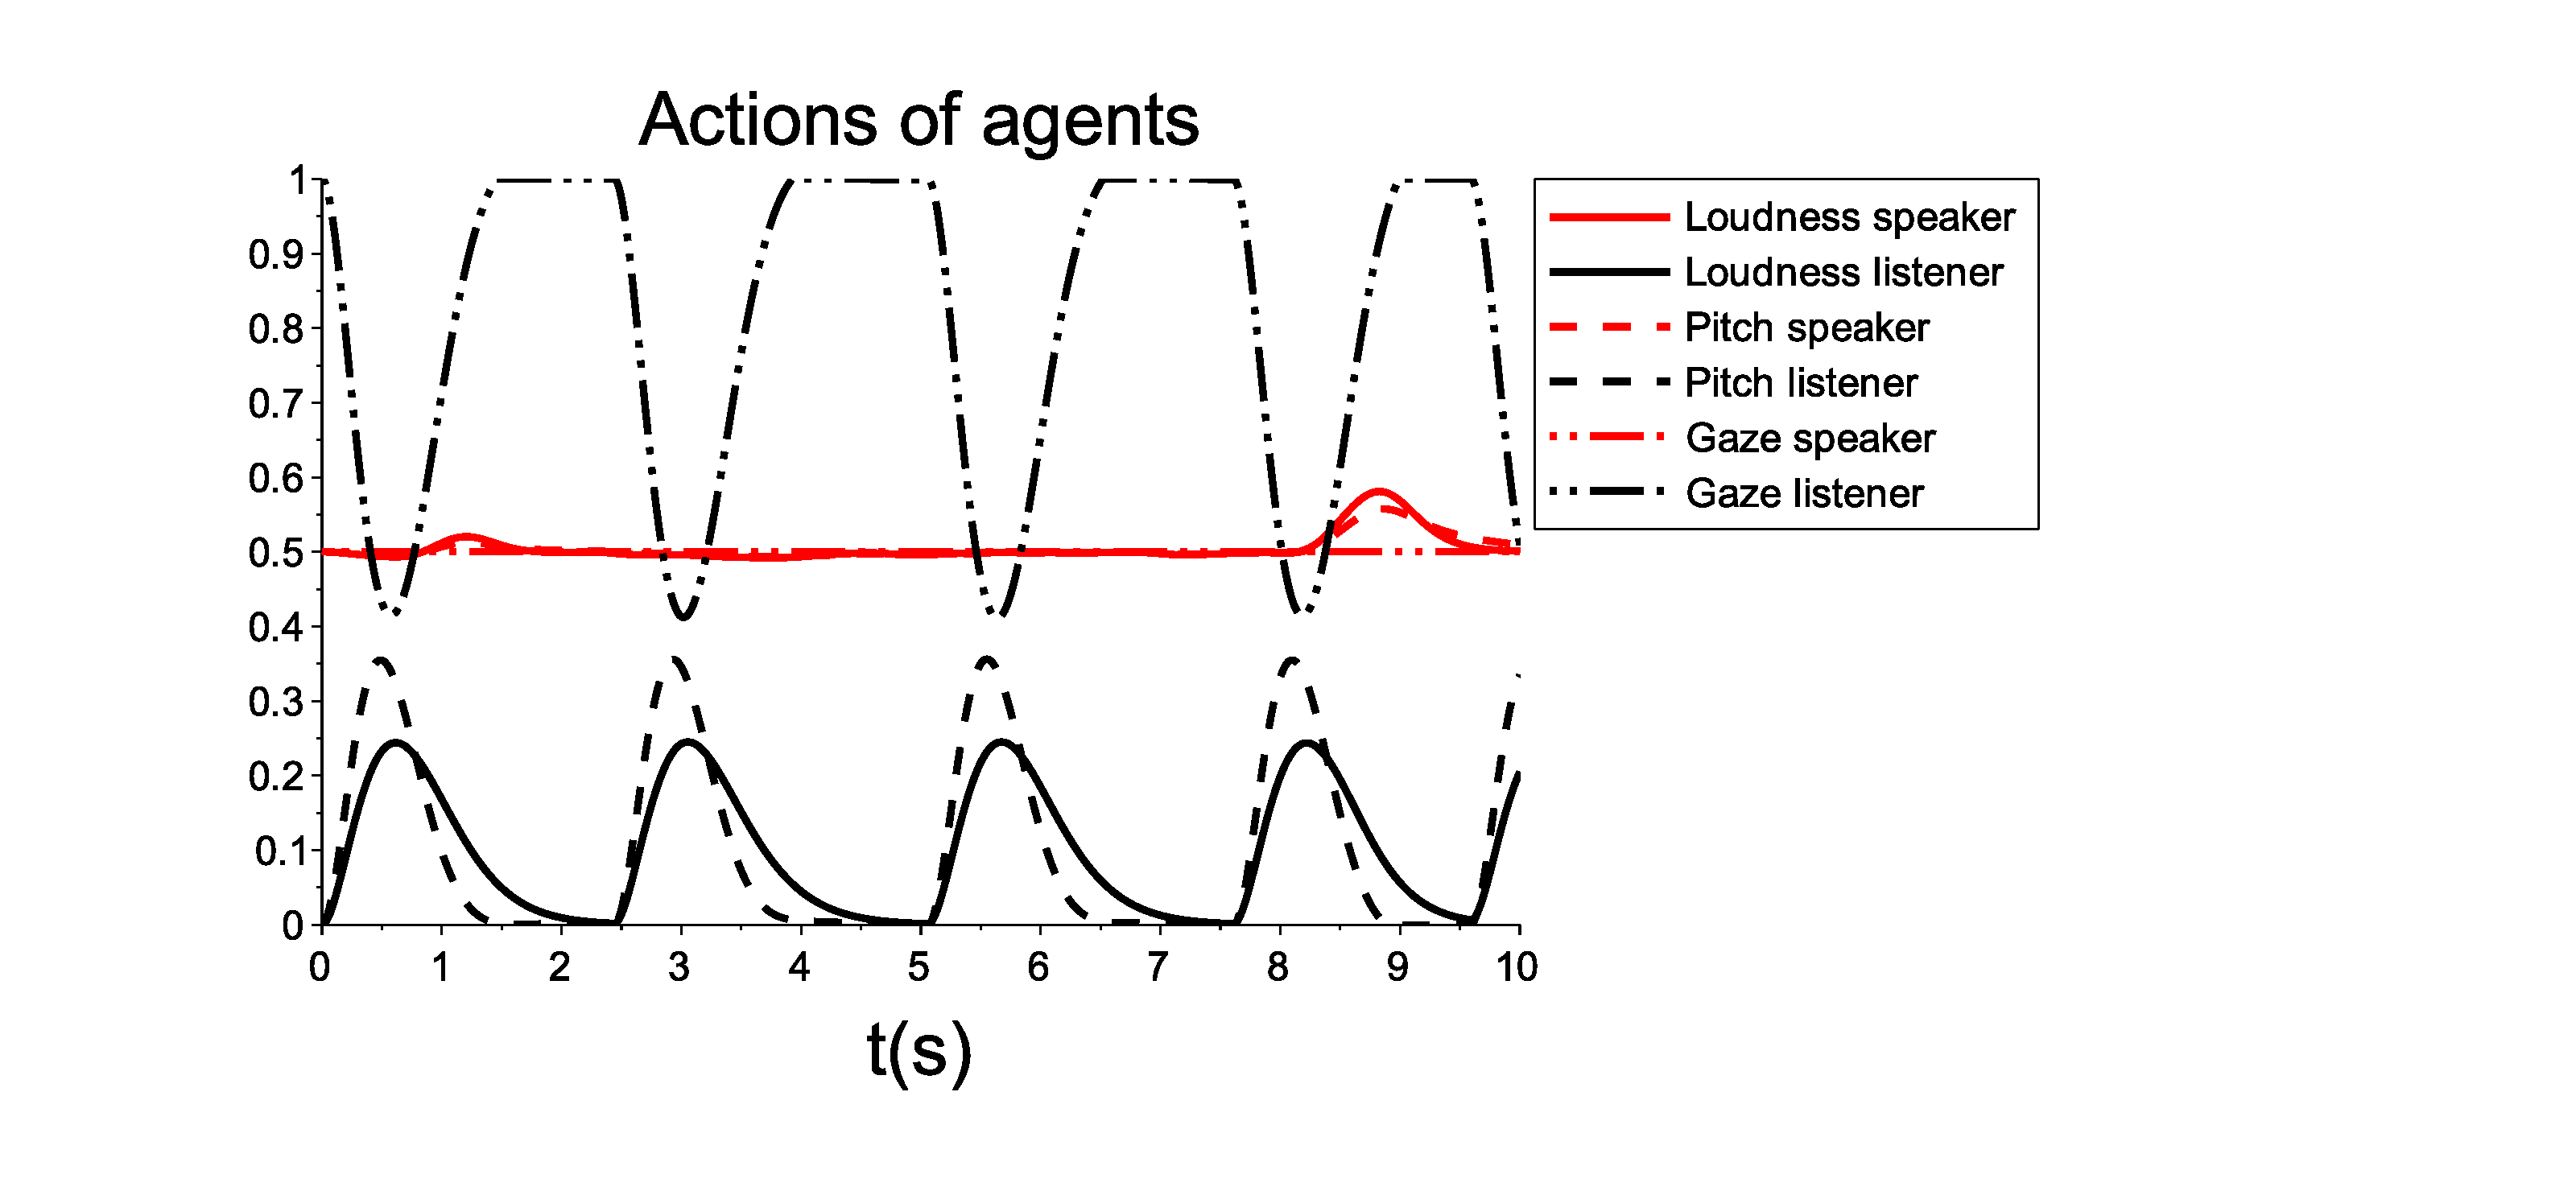
\includegraphics[width=\linewidth]{figure/adapt_all.pdf}
%   \caption{Conflictual situation where the participants have access to all of the three signals produced by the other participant.}
%   \label{adapt_all}
% \end{figure}

%We then analyzed the behavior of the participants when they could not perceive the gaze direction of their partner and had only access to the vocal modalities of the other participant's behavior.

\begin{figure}
  \centering
  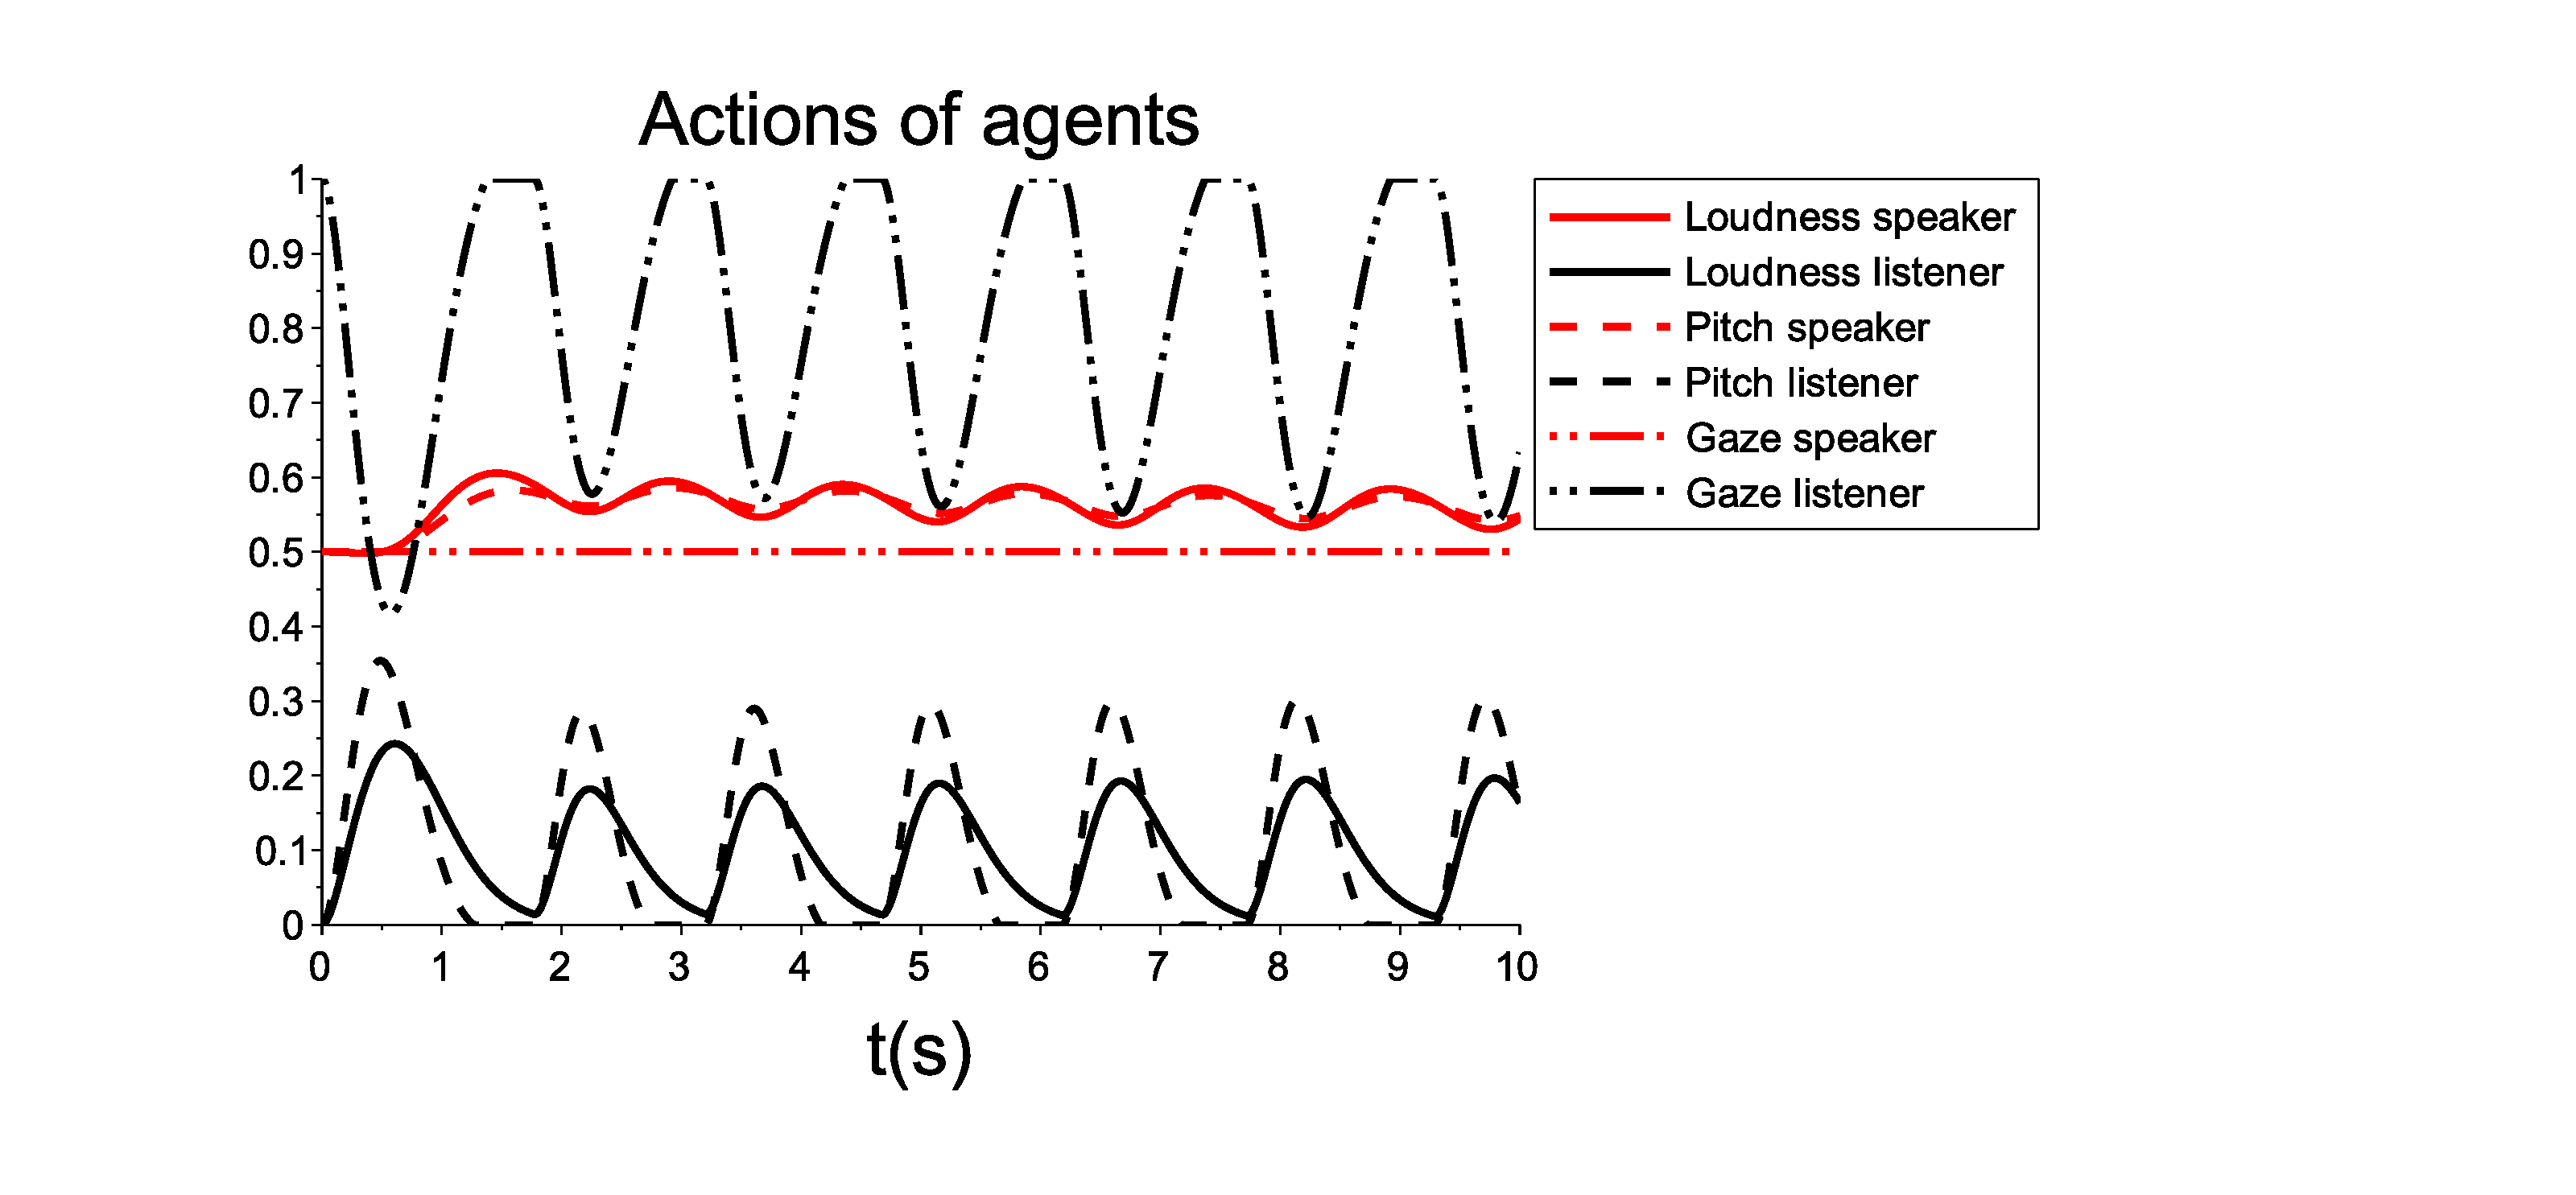
\includegraphics[width=\linewidth]{figure/adapt_nogaze.pdf}
  \caption{Conflictual situation where the participants do not have access to the gaze information of the other participant. Scenario S6.}
  \label{adapt_nogaze}
\end{figure}

%As shown on Figure \ref{adapt_nogaze}, 
%During S6, we observed a raise in the prosodic signals of the speaker. This was due to the joint influence of the volume and pitch raises of the listener, and to the current accumulation value, linked to the absence of the gaze information. 
In scenario S5, where participants exchanged the whole set of signals, the speaker's accumulation value raised but remained negative as the current listener attempted to take the turn but rapidly gave up. It was because the information conveyed by the listener's gaze evolved slowler than the prosodic information. Thus, at the beginning, the speaker did not perceive the cue in the gaze information indicating that the listener wanted to take the turn, diminishing consequently the variation of the accumulation value. 

In scenario S6, the accumulation value of the listener raised more rapidly and took more time to diminish in response to the lack of cues indicating that the speaker released the turn, resulting in a an agent raising more and longer its loudness and pitch. The fact that the loudness and pitch of the listener raised more impacted also the accumulation value of the speaker that raised more and became positive, that was not the case previously, resulting in an agent that raised more its own loudness and pitch. This raise impacted the accumulation value of the listener that diminished again, resulting in the listener giving up its turn-taking attempt. 

In addition, we simulated a situation where the participants perceived only the voice loudness, and we observed the same kind of adaptation: the speaker raising even more its loudness in response to the turn-taking attempts of the listener, as shown on Figure \ref{adapt_volume}.

\begin{figure}
  \centering
  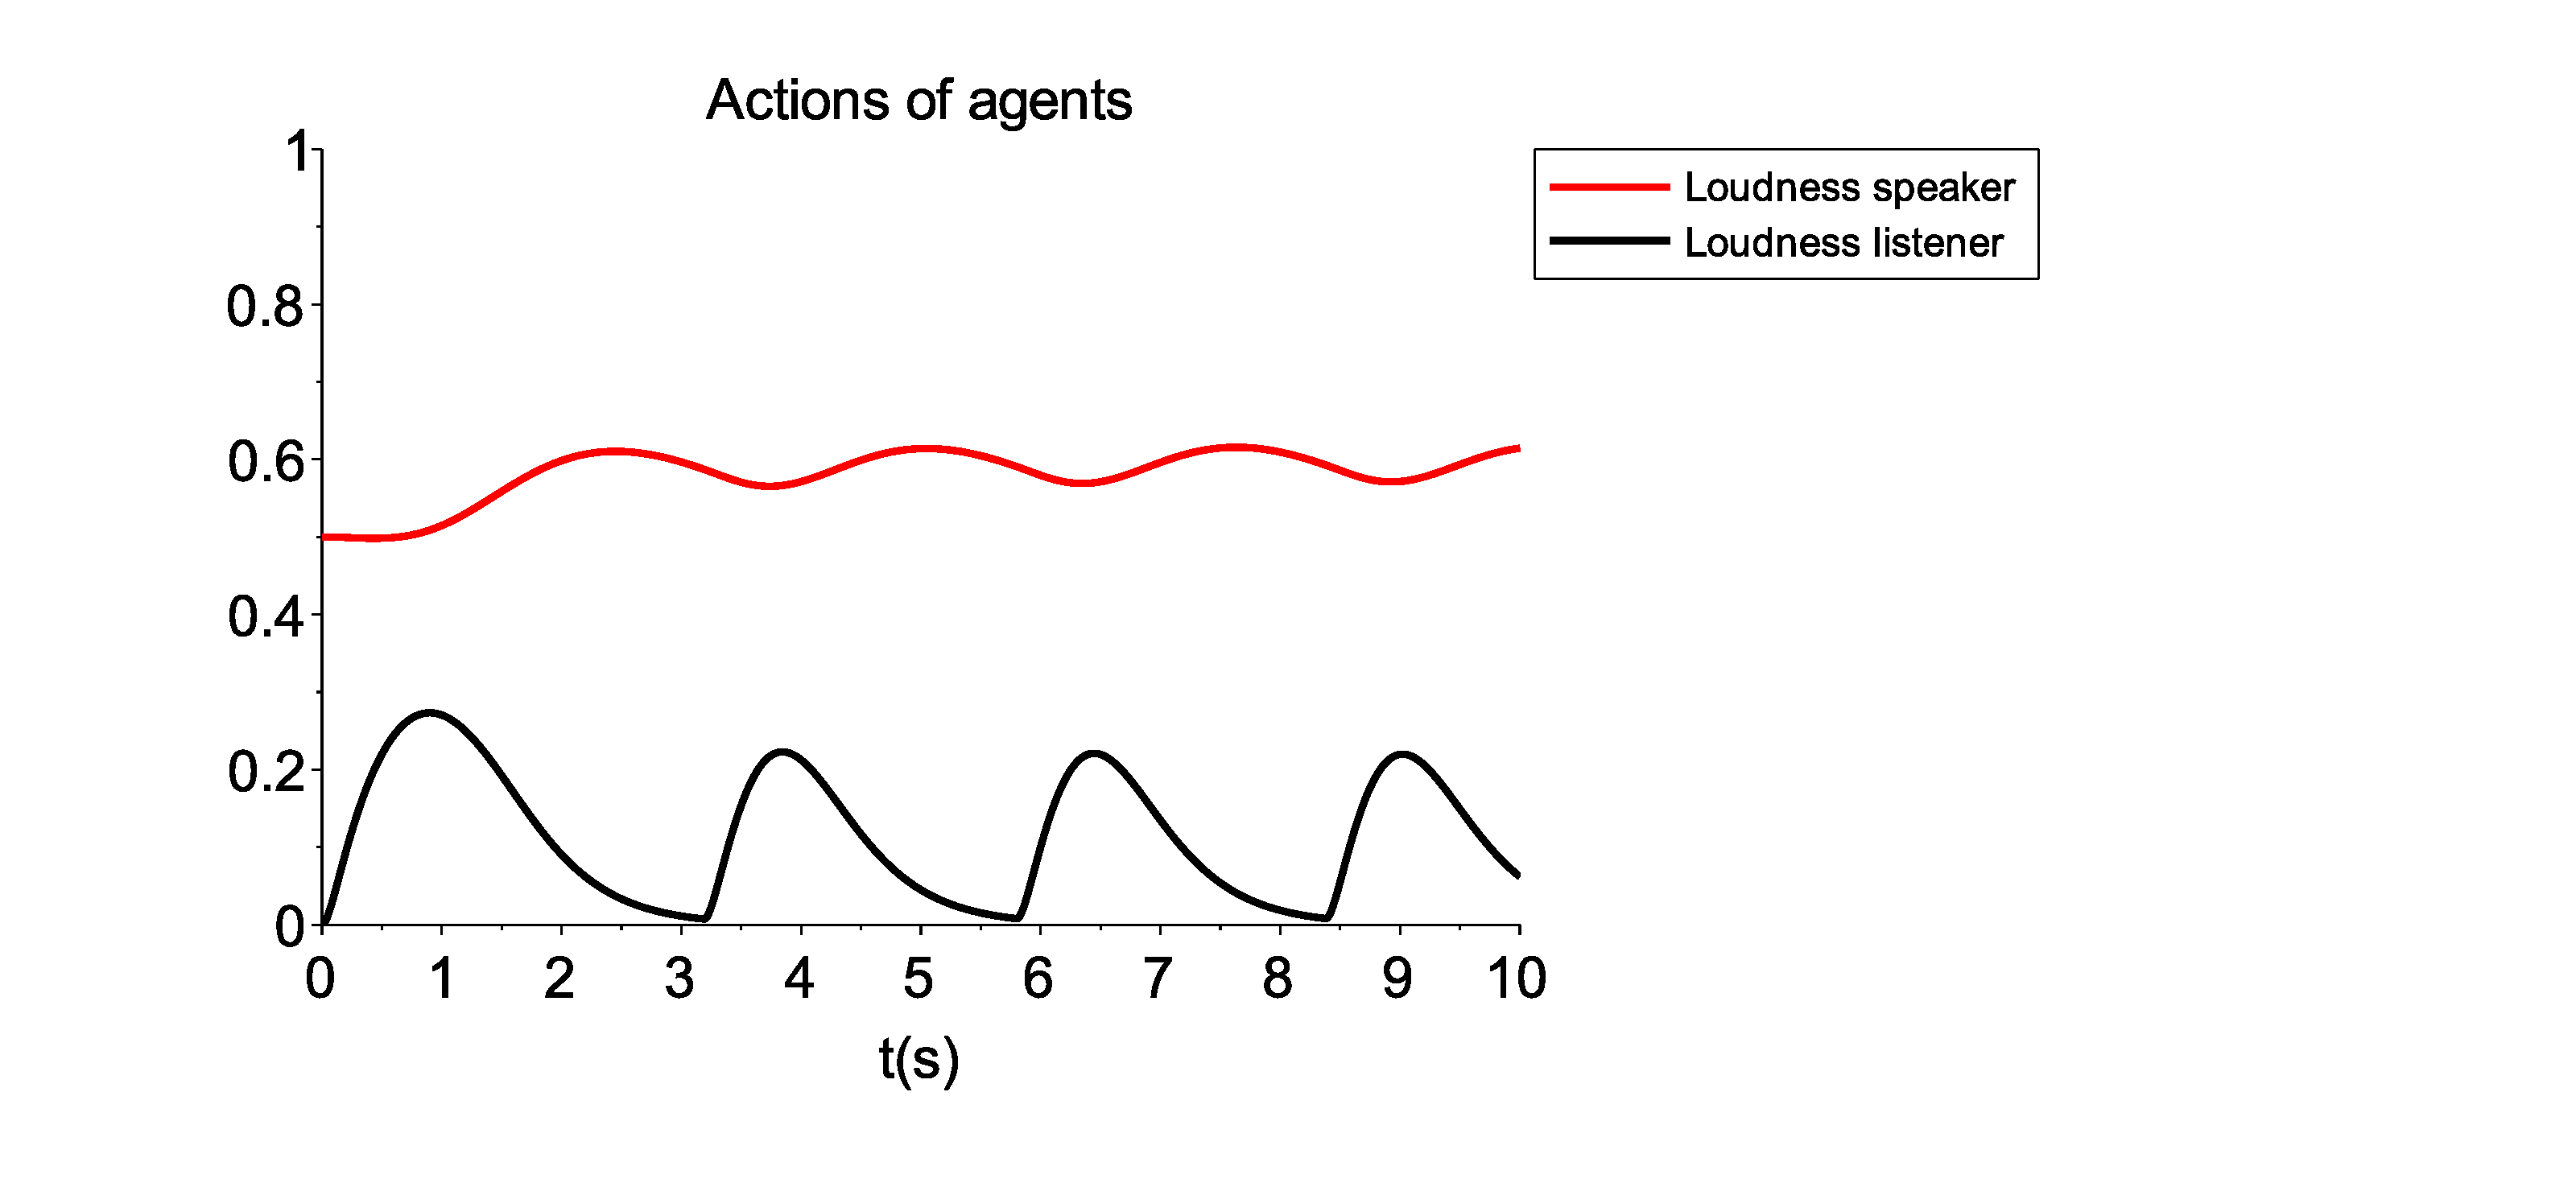
\includegraphics[width=\linewidth]{figure/adapt_volume.pdf}
  \caption{Conflictual situation where the participants have access only to the loudness produced by the other participant.}
  \label{adapt_volume}
\end{figure}

What is remarkable about these three contrasting scenarios is that the conflict durations did not vary significantly with the amount of signals handled by the agents. Interestingly, participants kept the coordination effective, and this was not totally due to the equations we formulated, but also to the manner participants varied their signals, accentuating their signal productions to compensate the lack of information in the environment. The adaptation of the agents is thus an emergent property of the interaction. Such mechanism is a great advantage for a turn-taking model between the agent and the user, as the adaptation of the agent is naturally done in the course of the interaction, without needing an explicit adaptation algorithm. Nevertheless, having the same adaptation properties in user-agent interactions necessitates that the user can also actively adapt to the situation. We explore this point in Section \ref{sec:eval}.